%% 
%% Copyright 2019-2021 Elsevier Ltd
%% 
%% This file is part of the 'CAS Bundle'.
%% --------------------------------------
%% 
%% It may be distributed under the conditions of the LaTeX Project Public
%% License, either version 1.2 of this license or (at your option) any
%% later version.  The latest version of this license is in
%%    http://www.latex-project.org/lppl.txt
%% and version 1.2 or later is part of all distributions of LaTeX
%% version 1999/12/01 or later.
%% 
%% The list of all files belonging to the 'CAS Bundle' is
%% given in the file `manifest.txt'.
%% 
%% Template article for cas-sc documentclass for 
%% single column output.

\documentclass[a4paper]{cas-sc}

% If the frontmatter runs over more than one page
% use the longmktitle option.

%\documentclass[a4paper,fleqn,longmktitle]{cas-sc}

%\usepackage[numbers]{natbib}
\usepackage[authoryear]{natbib}
%\usepackage[authoryear,longnamesfirst]{natbib}
\usepackage{dsfont}
\usepackage{array}
\usepackage{float}
\usepackage{placeins}
\usepackage{makecell} % add by shuyun
%\usepackage[utf8]{inputenc}
\usepackage{lineno,hyperref}
\usepackage{amsmath}
\usepackage{graphicx}
\usepackage[small]{caption}
\usepackage{subcaption}
\usepackage{array}
\usepackage{multirow}
\usepackage{multicol}
\usepackage{diagbox}
\usepackage{mathrsfs}
\usepackage{color}
\usepackage{booktabs}
\usepackage{soul}
\usepackage{mathspec}
\usepackage{xeCJK}
\setCJKmainfont{STKaiti}

%\setCJKmainfont[Mapping=tex-text]{STKaiti}
\usepackage[ruled, linesnumbered, vlined]{algorithm2e}

%\linenumbers

%%%Author macros
\def\tsc#1{\csdef{#1}{\textsc{\lowercase{#1}}\xspace}}
\tsc{WGM}
\tsc{QE}
%%%

% Uncomment and use as if needed
%\newtheorem{theorem}{Theorem}
%\newtheorem{lemma}[theorem]{Lemma}
%\newdefinition{rmk}{Remark}
%\newproof{pf}{Proof}
%\newproof{pot}{Proof of Theorem \ref{thm}}


\newcommand{\1}[1]{\mathds{1}\left[#1\right]}
\renewcommand{\floatpagefraction}{0.8}

\newcommand{\secref}[1]{Section \ref{#1}}
\newcommand{\figref}[1]{Figure \ref{#1}}
\newcommand{\eqnref}[1]{Eq. (\ref{#1})}
\newcommand{\exref}[1]{Example \ref{#1}}
\newcommand{\algoref}[1]{Algorithm \ref{#1}}
\newcommand{\tableref}[1]{Table \ref{#1}}
\newcommand{\socvec}{SocVec}
\newcommand{\argmin}{\operatornamewithlimits{argmin}}
\newcommand{\argmax}{\operatornamewithlimits{argmax}}
\newtheorem{example}{Example}
\newtheorem{lemma}{Lemma}
\newtheorem{definition}{Definition}
\newcommand{\cut}[1]{}
\newcommand{\ZY}[1]{\textcolor{red}{Zhiyi: #1}}

\begin{document}
	\let\WriteBookmarks\relax
	\def\floatpagepagefraction{1}
	\def\textpagefraction{.001}
	
	% Short title
	\shorttitle{A Token-based Transition-Aware Joint Framework for Multi-Span Question Answering}    
	
	% Short author
	\shortauthors{Z. Luo et al.}  
	
	% Main title of the paper
	\title{A Token-based Transition-Aware Joint Framework for Multi-Span Question Answering}  
	
	\author{Zhiyi Luo}[type=editor,auid=000,bioid=1,orcid=0000-0002-2206-1926]
	%\cormark[1]
	\ead{luozhiyi@zstu.edu.cn}
	\ead[url]{http://zhiyiluo.site}
	%\credit{Conceptualization of this study, Methodology, Software}
	
	\author{Yingying Zhang}
	\ead{272831920@qq.com}
	
	\author{Shuyun Luo}
	\ead{shuyunluo@zstu.edu.cn}
	\cormark[1]
	\cortext[mycorrespondingauthor]{Corresponding author}
	
	\address[mymainaddress]{School of Computer Science and Technology and the Key Laboratory of Intelligent Textile and Flexible Interconnection of Zhejiang Province, Zhejiang Sci-Tech University}
	\address[mysecondaryaddress]{No. 928, No. 2 street, Baiyang street, Qiantang New District, Hangzhou 310018, China}
	
	
	% % Here goes the abstract
	\begin{abstract}
		Multi-span question answering has gained prominence as it aligns more closely with real-world user requirements compared to single-span question answering. The utilization of pretrained language models has shown promise in improving multi-span question answering, particularly for factoid questions that necessitate entity-based answers. However, existing methods tend to overlook critical information regarding answer span boundaries, resulting in limited accuracy when generating descriptive answers. To address this limitation, we propose TOAST, a novel joint learning framework specialized in token-based neighboring transitions that capture answer span boundaries through adjacent word relations. Our approach extracts high-quality multi-span answers and is general-purpose, applicable to both alphabet languages like English and logographic languages like Chinese. Furthermore, we introduce CLEAN, a comprehensive open-domain Chinese multi-span question answering dataset, which includes a substantial number of descriptive questions. 
		Extensive experiments demonstrate the superior performance of TOAST over previous top-performing QA models in terms of both EM F1 and overlapped F1 scores. Specifically, the TOAST models, leveraging  $\text{BERT}_{base}$ and $\text{RoBERTa}_{base}$, achieve substantial  improvements in EM F1 scores, with increments of 3.03/2.13, 4.82/3.73, and 16.26/11.53, across three publicly available datasets, respectively. 
		
	\end{abstract}
	% 
	% Use if graphical abstract is present
	%\begin{graphicalabstract}
	%\includegraphics{}
	%\end{graphicalabstract}
	% 
	% Research highlights
	%\begin{highlights}
	%\item The paper proposes a novel joint learning framework called TOAST, which specializes in token-based neighboring transitions to capture the boundary information of answer spans through adjacent word relations for multi-span question answering.
	%\item TOAST extracts high-quality multi-span answers and is general-purpose, applicable to both alphabet languages like English and logographic languages like Chinese.
	%\item The paper creates a new Chinese reading comprehension dataset, consisting of both single-span and multi-span answers, with a broad-coverage of types of open-domain questions and demonstrates that incorporating the span boundary information via the awareness of adjacent word relations improves strong baselines on three multi-span question answering datasets.
	%\end{highlights}
	
	% Keywords
	% Each keyword is seperated by \sep
	\begin{keywords}
		Reading comprehension \sep Multi-span question answering \sep  Pretrained language models \sep Multitask learning  \sep Chinese datasets 
	\end{keywords}
	%Reading comprehension \sep
	%\sep Neural networks
	% \keywords{multi-span question answering, reading comprehension, chinese datasets, joint learning, neural networks}
	\maketitle
	
	
%	\section{Introduction}
\label{sec:intro}

Let's cite a paper~\cite{DBLP:conf/aaai/PangLGXSC19}.

In summary, the main contributions in this paper are as follows:
\begin{itemize}
	\item We employs a automatic data augmentation framework using Large Language Model \((LLM)\) as a knowledge source and a extra content supplement to linearize relevant information and possible continuation from LLM as texts, then inject them into original contexts. 
	\item We develop a series of prompt templates designed for interacting with ChatGPT to acquire comprehensive explanations of numerous entities. These templates ensure that the formats of the responses provided by ChatGPT are highly parseable and well-structured.
	
\end{itemize}

%The introduction should briefly place the study in a broad context and highlight why it is important. It should define the purpose of the work and its significance. The current state of the research field should be reviewed carefully and key publications cited. Please highlight controversial and diverging hypotheses when necessary. Finally, briefly mention the main aim of the work and highlight the principal conclusions. As far as possible, please keep the introduction comprehensible to scientists outside your particular field of research. Citing a journal paper \cite{ref-journal}. Now citing a book reference \cite{ref-book1,ref-book2} or other reference types \cite{ref-unpublish,ref-communication,ref-proceeding}. Please use the command \citep{ref-thesis,ref-url} for the following MDPI journals, which use author--date citation: Administrative Sciences, Arts, Econometrics, Economies, Genealogy, Humanities, IJFS, Journal of Intelligence, Journalism and Media, JRFM, Languages, Laws, Religions, Risks, Social Sciences, Literature.
%%%%%%%%%%%%%%%%%%%%%%%%%%%%%%%%%%%%%%%%%%

\section{Introduction}
\label{sec:introduction}

Extractive question answering, also commonly referred as the task of reading comprehension, which aims to answer a user's question by finding short text segments (i.e., {\em spans}) from the given context, has been actively studied and achieved rapid progress in recent years.
Benefiting from the sophisticated industrial search engines and the vast amount of text collections on the web, 
high-quality contexts relevant to the user questions can be effectively retrieved to construct the datasets.
As a result, the answers directly drawn from the high-quality contexts are expressive enough.
Hence, existing datasets and models~\citep{DBLP:conf/emnlp/DasigiLMSG19,li2022multispanqa,lee2023liquid,DBLP:journals/ipm/Liu0GC23}, cast reading comprehension as an \emph{extractive} task that is easy to learn.

Most previous work~\citep{rajpurkar2016squad,rajpurkar2018know,yang2018hotpotqa,zaheer2020big} restricts the answer extracted from the context to a single text span 
which can only satisfy limited real-world open-domain questions. 
For example, as shown in \tableref{tab:intro} (the left example), the complete answer to a question could consist of a series of non-contiguous spans, 
or even the question itself could have multiple intents, 
where the answer to each intent is composed of one or more spans drawn from the input.
Hence, the models of multi-span question answering have significant utility to users. 
Recently, ~\cite{segal2020simple} cast the multi-span extraction as a sequence tagging task, 
predicting whether each token is part of an answer. 
~\cite{li2022multispanqa} captured the global information by integrating two sub-tasks of predicting the number of spans to extract and the answer structure annotated in their proposed dataset. 
Benefiting from nowadays pretrained models (e.g., BERT~\citep{kenton2019bert}, RoBERTa~\citep{liu2019roberta}), 
the above neural approaches 
have achieved promising performance on answer span extraction,  
especially for factoid questions where the expected answers are \emph{entities} (e.g., \emph{Person} and \emph{Location}).

However, existing systems fail to carefully consider span boundaries according to the information need of the question, 
and thus have very limited capabilities of 
precisely drawing a \emph{description} answer, for example, 
the answer spans of ``饮食护理(diet and care)'' and  ``适当地带它们出去运动一下(take them out for some exercises)''
as shown in \tableref{tab:intro}, from the input.
Moreover,  in the construction of existing datasets, 
user question candidates are constrained 
by the organization way of the document collection 
where the relevant contexts are retrieved from. 
For example, Wikipedia, the most widely used document collection 
for context retrieval, organizes articles using entities.
The problem is that a \emph{semantic gap} exists between the real context of what users want to ask and the entity-based articles (i.e. single Wiki page). 
Backed by the document collection of Wikipedia, 
existing datasets include most types of the factoid questions,
whereas they exclude many questions that can not be answered from a single 
article of an entity.
% =====  draw a figure here ====
\begin{table}[width=\textwidth,cols=4,pos=h]
	%	\centering
	\caption{Examples of questions and answers.}
	\begin{tabular*}{\tblwidth}{c|c|c} \hline
		Dataset   & CLEAN   &  MultiSpanQA \\ \hline
		Question  &  {\makecell[l]{
				如何养好约克夏犬?
				\\ (How to raise a Yorkshire terrier?)}} & Who wrote the song if you could see me now? \\ \hline
		Context  & {\makecell[l]{想要养好约克夏对于它们的{\color{blue}饮食护理}都要做好,\\
				由于它们所需的运动量并不是特别大,所以一般\\
				在家里就可以,不过还是要{\color{blue}适当地带它们出去运}\\
				{\color{blue}动一下},这样它们能够生长的更好。\\
				(...
				must do a good job in their {\color{blue}diet and care.}\\
				... but it is still necessary to
				{\color{blue}take them out for}\\
				{\color{blue}some exercise} so that they can grow better.)}} 
		&  {\makecell[l]{
				``If You Could See Me Now'' is a 1946 jazz\\
				standard, composed by {\color{blue}Tadd Dameron}. He\\
				wrote it especially for vocalist Sarah\\
				Vaughan, a frequent collaborator. Lyrics\\
				were written by {\color{blue}Carl Sigman} and it became\\
				one of her signature songs, inducted into\\
				the Grammy Hall of Fame in 1998.}}
		\\ \hline
		Answer & {\makecell[l]{Segment1:饮食护理(diet and care)\\Segment2:适当地带它们出去运动一下\\(take them out for some exercise)}} &
		{\makecell[l]{Segment1: Tadd Dameron\\
				Segment2: Carl Sigman}}\\ \hline
	\end{tabular*}
	\label{tab:intro}
\end{table}

Following the above observations, we in this paper propose a novel approach to explicitly model the implicit \emph{neighboring transitions} 
via the adjacent word (or token) relations, 
which are both semantically and syntactically informative for span boundaries identification. 
This approach captures the intuition that the span boundary is produced in-between adjacent words. 
We indicate neighboring transitions in-between
as five types of relations.
Then, we jointly learn the sequence tagging task 
together with the  adjacent word relation classification task 
evolved from the span boundary identification, 
considering whether each token is part of an answer 
and which span each token belongs to accordingly. 
With the awareness of adjacent word relations, 
we incorporate the information of span boundaries in a multi-task learning manner.
Furthermore, in order to ameliorate the observed limitation of previous datasets, 
which including more real-world open-domain questions, 
we create a new dataset (in Chinese) in a more natural manner, 
extracting question-context pairs from a large-scale knowledge Q\&A sharing platform (i.e., BaiduZhidao\footnote{https://zhidao.baidu.com/}) instead of Wikipedia. 


In summary, the main contributions in this paper are as follows:
\begin{itemize}
	\item We create a new reading comprehension dataset named CLEAN~\footnote{We intend to make CLEAN 1.0 dataset publicly avaiable at http://zhiyiluo.site/misc/clean\_v1.0\_sample.json for future work in this research area.} that consists of both single-span and multi-span answers, covering a wide range of open-domain question topics. 
	CLEAN overcomes the constraints imposed by previous datasets by incorporating carefully crafted long answers as contexts, effectively bridging the semantic gap with the insights provided by respondents. 
	\item We propose a novel approach for multi-span reading comprehension,  where we explore implicit neighboring transitions using adjacent word relations, effectively capturing both semantic and syntactic information pertaining to the boundaries of answer spans.
	
	\item We demonstrate that incorporating the span boundary information via the awareness of adjacent word relations improves strong baselines on three multi-span question answering datasets (both English and Chinese).
\end{itemize}

%	\section{Our Approach}

\begin{figure*}[h]
	\centering
	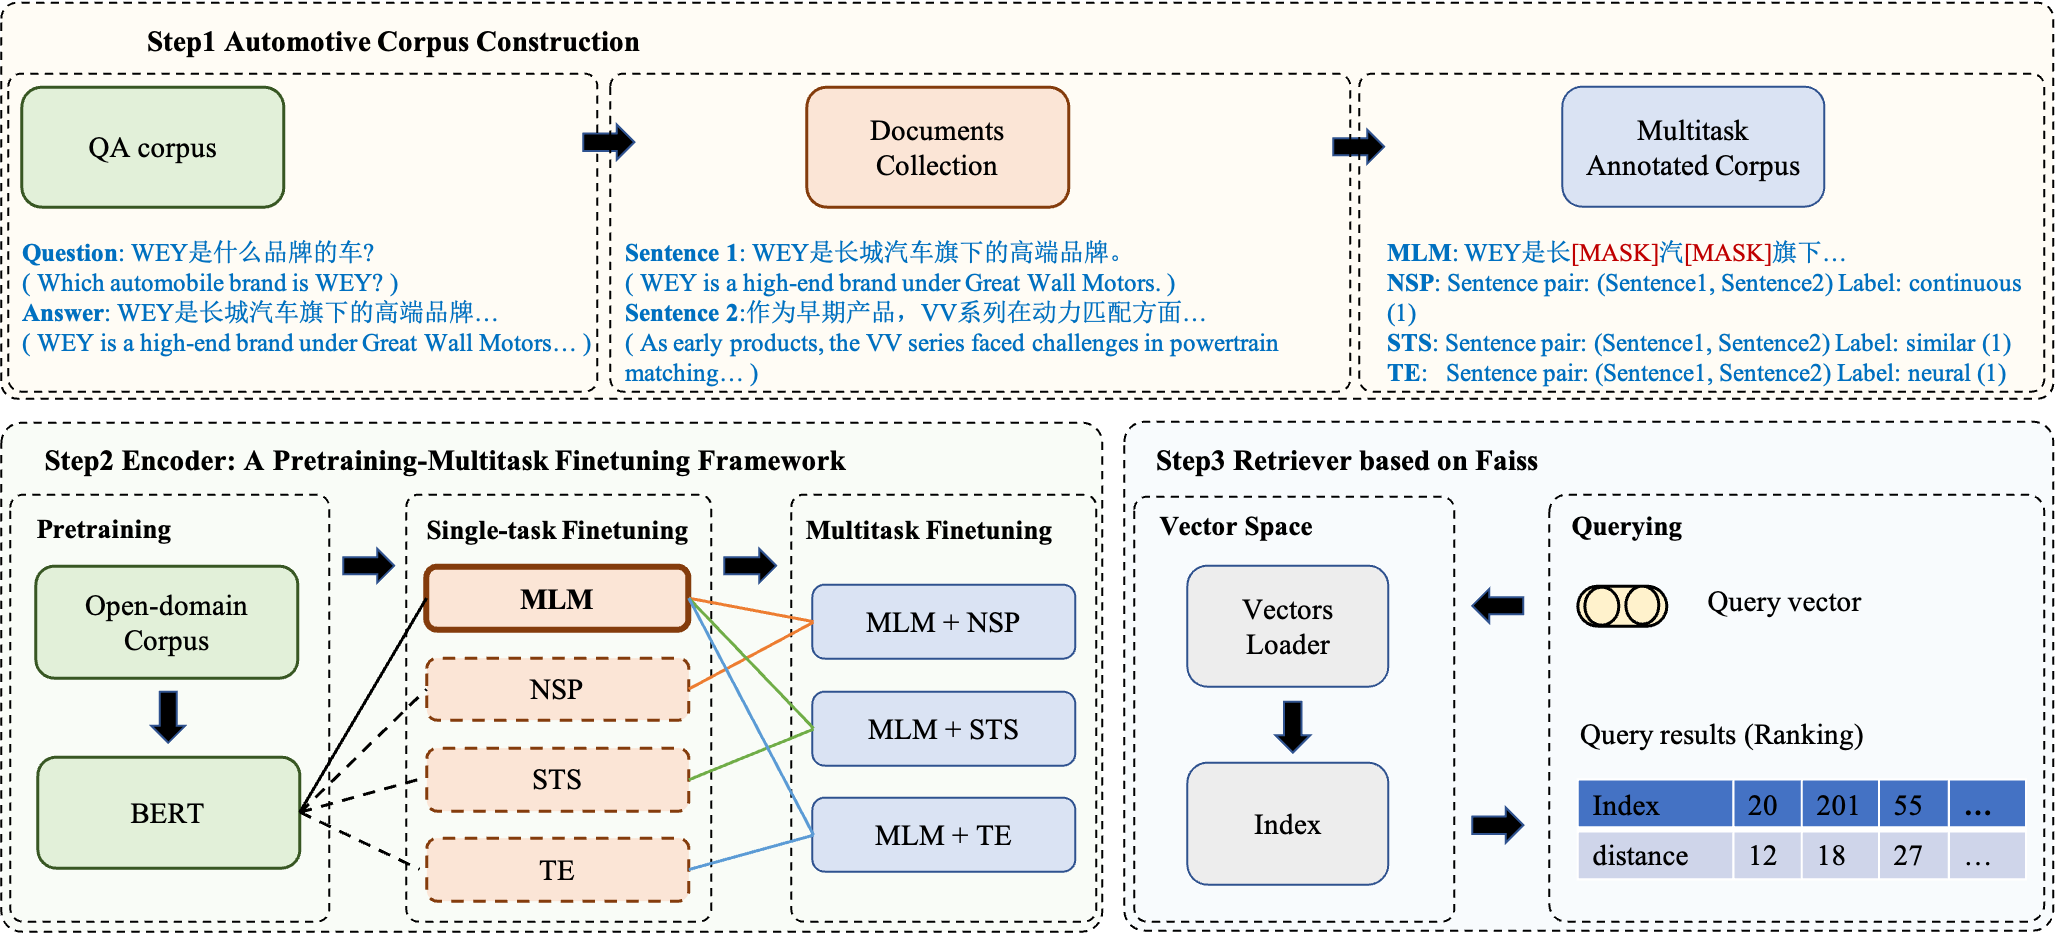
\includegraphics[width=18cm]{overview.png}
	\caption{An overview of our automatic information augmentation framework. \textbf{(a) Step 1}: Interact with ChatGPT to Get Auxiliary Information. \textbf{(b) Step 2}: Distilling the Information and Injecting Them into Context \textbf{(c) Step 3}: Input the Augmented Context into Tagging Model}
	\label{fig:overview}
\end{figure*}   


%\unskip
Existing extractive multi-span question answering models exhibit subpar performance in handling ambiguous words, complex proper nouns (such as film and song titles), numerical values, and long descriptive answers. The main reasons for these shortcomings can be categorized into three aspects:

\textbf{Ambiguous Words}: The real world is replete with words that have a single form but multiple meanings, which heavily depend on the context. For instance, the word ``Cameron" could refer to a famous director or a former British Prime Minister, depending on the context. The specific meanings of such words often appear infrequently in training corpora, making them difficult to learn.

\textbf{Numerical Values}: In contrast to ambiguous words, numerical values have a single meaning but can be represented in various forms. For example, "22.5 billion years" can also be expressed as "cosmic years".

\textbf{Multi-span Answers}: In extractive multi-span question answering tasks, the model needs to grasp the overall relationship of multi-span answers in the context, such as parallelism and progression.These challenges require the model to possess a high level of comprehensive understanding ability and knowledge about language and the world. 

Leveraging large language models to parse question-answering data and inject auxiliary knowledge into the model can promote the integration of the model's latent world knowledge and specific domain knowledge in the paragraph, thereby enhancing the model's performance. Thus, we use GPT-3.5-turbo to generate entity annotations, entity association analysis, and content continuation for each question-answering paragraph as auxiliary information for the model:

\textbf{Context Supplementary}: By inserting explanations of entities in the form of annotations after the main entities or concept words in the question and paragraph, this method helps the model capture the actual meaning of ambiguous words in specific contexts. It provides direct information prompts for low-frequency meanings or low-frequency words, achieving entity or concept alignment in the question-answering system.

\textbf{Context Enrichment}: By integrating entity association analysis and content continuation with the original question-answering text to form new paragraphs based on knowledge enhancement, this method captures the inherent associations between words or entity concepts with the same meaning but different forms. On one hand, it parses the logical relationships between other entities using entity relationship analysis. On the other hand, it extends the original paragraph information using content continuation, introducing more external knowledge while helping the model understand the overall content direction of the paragraph, thereby enhancing the model's comprehension ability.


Overall,we design an automated knowledge enhancement method for multi-span question answering tasks, which interacts with large language models based on templates. This method is applicable to all question answering models or frameworks. It is universally applicable to any other downstream tasks that contain paragraph data, without the need for any complex calculations. In the following sections, we will provide a detailed introduction to each specific module of this process.

\subsection{Construction of Prompt Template}
\label{sec:prompt_construction}
\begin{figure*}[h]
	\centering
	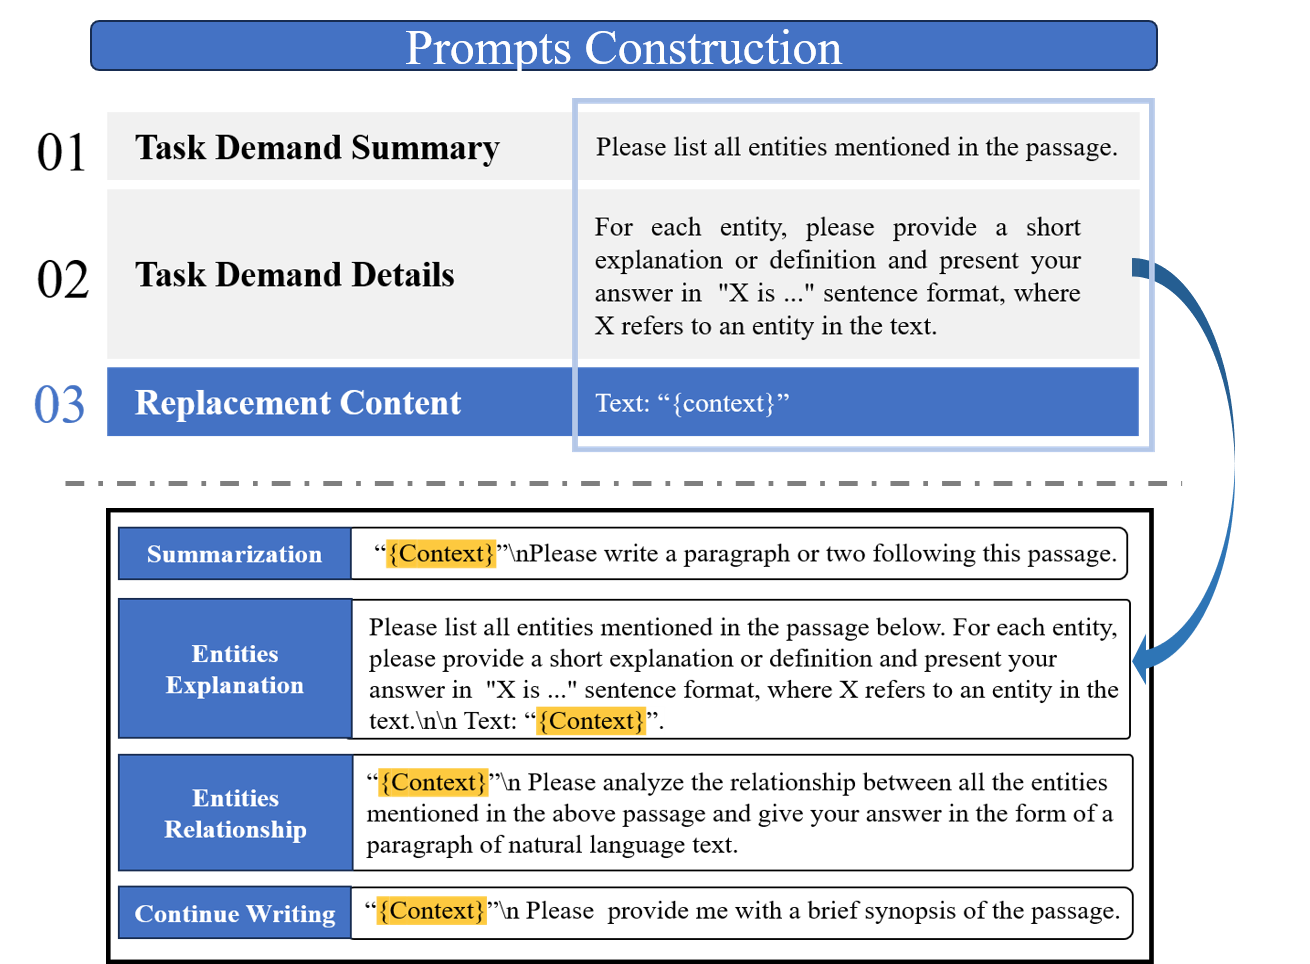
\includegraphics[width=14.5cm]{Prompts_construction.png}
	\caption{Prompt Templates and it's Construction}
	\label{fig:prompt_template}
\end{figure*}   

The quality and format of the content produced by LLMs depends greatly on the prompts. Hence, it is necessary to clarify the format and content requirements of the outputs in advance, and to refine the templates that meet the expectations through extensive evaluation.
For entity relationship parsing and textual continuation, it would be better to ensured that the the output is a natural paragraph, to facilitate the automatic splicing of the enriched knowledge with the initial paragraphs,which is consistent with encoder's natural input format.
Regarding knowledge of entity explanation, the inserted knowledge fusion method requires a parsable and structured outputs for automatic recognition and segmentation of entities and their explanations in post-processing, as well as inserting explanation behind the description of matched entity in initial context.

Concretely, by clearly specifying the form and requirements in the prompts, especially for entity relationship parsing and contextual continuation, which need to be formulated in the form of natural statements, the targeted enhanced knowledge can be obtained more easily.
Furthermore, to obtain well-structured results for complex model interactions, like entity explanations, we utilize a set of corresponding hint templates to construct the process, which has proven to be useful for interactions that require semi-structured answers through verification. 

Eventually, the template is piloted to clarify any ambiguous requirements in the template to confirm an accurate understanding of the LLMs (e.g., adding at the end of the prompt, ``Please return the answer in the following form, being careful not to repeat it: \textbackslash n\textbackslash nA is .....")  In addition, to avoid omission or confusion of requirements due to the length of the prompt text, specific principles should be reiterate in a separate paragraph.

\subsection{Information Injection}

To incorporate enhanced knowledge into the original data (comprising questions and paragraphs) pertaining to entity interpretation, a methodology involving the insertion of explanations is employed. Specifically, the process begins with the automated script parsing of entity interpretation data. This script, on one hand, utilizes regular expressions to analyze the structure of the majority of sentences, while on the other hand, for a limited subset of sentences that deviate from the template specifications, employs Spacy's Semantic Dependency Analysis model to identify entities and their corresponding interpretations.

Upon obtaining the ``Entity-Entity Interpretation" knowledge base for each question-and-answer data, a subsequent scan of the original context is conducted. For each entity that exists in the dataset's library of entities and their explanations, the corresponding explanation is inserted immediately following the entity, enclosed within parentheses. This meticulous approach ensures that the augmented text, enriched with knowledge, retains its natural sentence or paragraph flow. For instance, a resulting sentence might appear as follows: ``How long does it take for the Milky Way (Milky Way: The galaxy that contains our Solar System and is home to billions of stars.) to rotate?" 

\label{sec:information_injection}
\begin{figure*}[h]
	\centering
	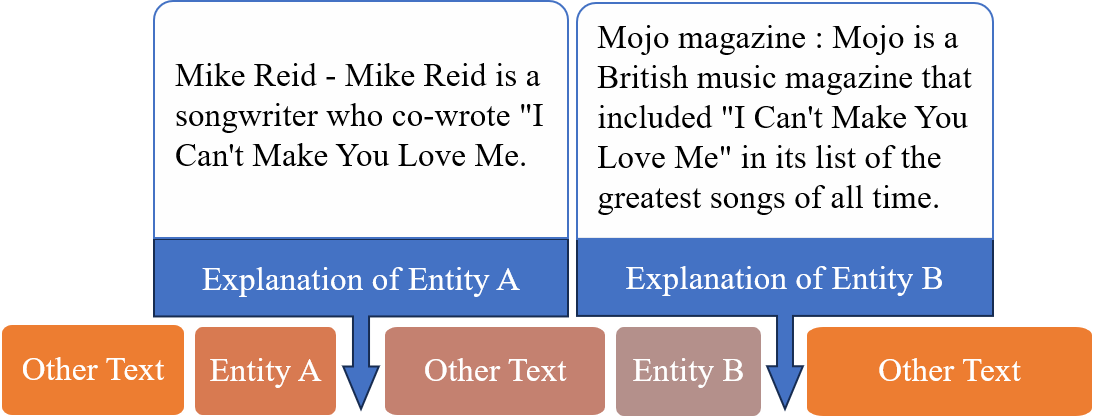
\includegraphics[width=10cm]{EntityInsert.png}
	\caption{The Process of Inserting Entity Explanation into Context}
	\label{fig:entity_insertion}
\end{figure*}

For the incorporation of enhanced knowledge related to entity relationship analysis and content continuation, a method of random slicing and concatenation based on length ratios is employed to infuse the augmented knowledge into the original paragraphs. Initially, the ratio of the average length of the augmented knowledge text to that of the original paragraph is calculated. Subsequently, at the model's input layer, the original input data is segmented into text fragments of length of \textit{512 * average original length / (average original length + average augmented text length)}, and the augmented text is also segmented into text fragments of length of  \textit{512 * average augmented text length / (average original length + average augmented text length)}. Then, random selections of augmented text fragments are made and concatenated into the middle of each original text fragment. Finally, this concatenated longer text is fed into the model in a sliding manner to ensure comprehensive interaction between the original data and the augmented data at lower layers of the model, as illustrated in Figure~\ref{fig:random_concatenate}.



\begin{figure*}[h]
	\centering
	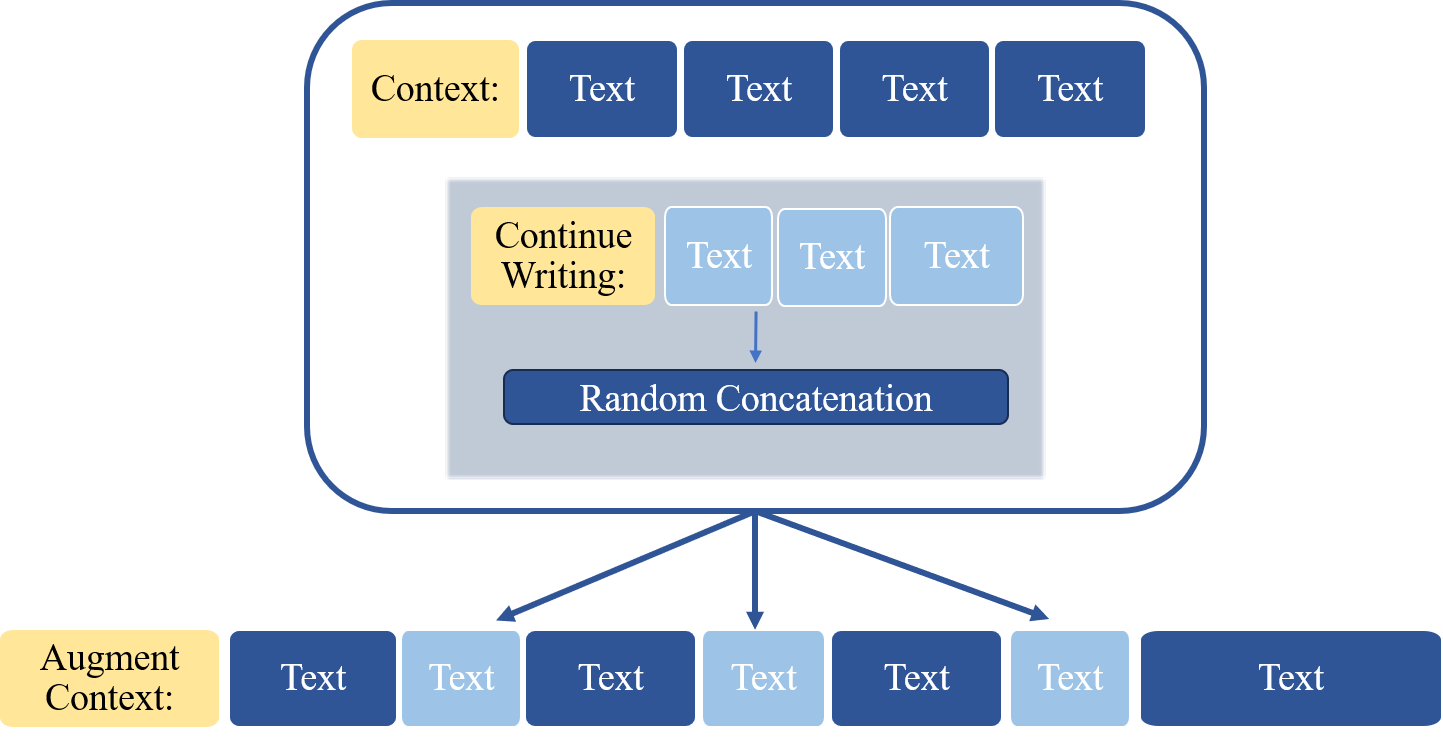
\includegraphics[width=10cm]{RandomConcat.png}
	\caption{The Process of Concatenation of Original Context and Auxiliary Information}
	\label{fig:random_concatenate}
\end{figure*}  

\subsection{Information Integration}
\label{sec:information_integration}
In addition to the aforementioned three types of information, we seek more valuable enhanced information by requesting summaries for each question-context pair from Large Language Models (LLMs). We then extract entities mentioned in the summaries to capture those highly relevant to the core context. Moreover, recognizing the intrinsic connection between entity explanation and entity relationship parsing, we categorize them as complementary information for context enrichment, with context continuation serving as supplementary information. This approach aims to augment the model's internal text-parsing knowledge with external world knowledge through enhanced information. 

To further investigate the efficacy of multi-information integration, leveraging enhanced information derived from Large Language Models (LLMs), we employ two distinct approaches to combine entity knowledge and context continuity. The first approach involves the incorporation of all information within the original context, with each type of information undergoing individualized knowledge injection. The second approach, referred to as "bagging," treats models trained on diverse information sources as voters. For each query, we employ all model predictions for token-level BIO labeling within the context, determining the final prediction through a majority vote. In cases of tie-breaking, we prioritize the logits' magnitude to ascertain the ultimate prediction.


%\section{Tasks and Datasets}
\section{Preliminary}
\label{sec:preliminary}
% 1.30  10:20 - 13:00  0.5页
In this section, we present the problem statement and then introduce the datasets. 
%\subsection{Task}
%\label{sec:tasks}
%Information retrieval based question answering (IR-based QA) systems consist of two components: \emph{retriever}  and  \emph{reader}. 
%The reading comprehension (RC) task focuses more on building the \emph{reader} model since the construction of the RC dataset already utilizes the \emph{retriever} component  explicitly or implicitly.
%Thus, we formulate the problem of multi-span question answering as a task of multi-span extraction on the basis of the RC datasets. The objective of the task is to extract one or more answer spans based on the input question and context.
\subsection{Problem Statement}
\label{sec:problem}
We formulate the problem of multi-span question answering as a task of multi-span extraction on the basis of the reading comprehension (RC) datasets. The objective of the task is to extract one or more answer spans based on the input question and context.

Formally, given an input question represented as a sequence of words 
$q=(q_1, q_2, ..., q_n) \in \mathcal{V}$, and an input context $c$, associating to $q$, 
which is also represented as a sequence of words $c=(c_1, c_2, ..., c_m)\in \mathcal{V}$, where $\mathcal{V}$ refers to the vocabulary, 
the objective of the system is to extract one or more spans as the answer $a$, 
say $l$ spans, $a = [a_1, a_2, ..., a_l]$ from the context $c$,
where the $i$-th span $a_i$ is a sequence of words $a_i=(c_{i_s}, c_{i_s+1}, ..., c_{i_e})$, 
ranging from the start position $i_s$ to its end position $i_e$. Note that the extracted answer spans should be neither duplicated nor overlap with each other. That means, for any $i, j$ where $i$ < $j$, $i_e < j_s$ holds. 
%Following previous studies, we regard the problem as a sequence tagging task.
%We also build an auxiliary task incorporating token-based transition knowledge to capture 
%the information of span boundaries, and jointly learn the sequence tagging task as well as the transition classification task.

Evaluation are exact match and partial match with any of the reference answer strings after minor normalization such as lowercasing, following evaluation scripts from~\cite{li2022multispanqa}.

\subsection{Datasets}
\label{sec:predata}
In this work, we conduct the experiments on three RC datasets, ranging from two English datasets and one proposed Chinese dataset for multi-span question answering. 

The latest dataset, MultiSpanQA, focus on multi-span questions, which is derived from Natural Question (NQ) ~\citep{DBLP:journals/tacl/KwiatkowskiPRCP19}, a large-scale open domain QA dataset. It also has an expanded variant by introducing single-span and unanswerable questions, namely MultiSpanQA (expand). 

In MultiSpanQA and MultiSpanQA (expand), the questions are derived from real queries issued to the Google search engine. Each question is paired with a context extracted from a retrieved Wikipedia page. However, it is important to acknowledge that Wikipedia pages are structured around entities, which may not fully align with the intentions of real-world open-domain questions, especially those that are non-factoid in nature. This entity-centric organization of Wikipedia pages introduces a semantic gap between the content and the intended meaning of real-world open-domain questions.
As a result, existing RC datasets like MultiSpanQA are limited to questions  that primarily revolve around entities, allowing for the extraction of concise spans from a single Wikipedia page as answers.
Moreover, there is a noticeable scarcity of publicly available open-domain multi-span QA datasets in the Chinese language. Although recently proposed CMQA~\citep{DBLP:conf/coling/JuWZZ0022} is one such dataset, it primarily focuses on a new task of conditional question answering, which may not directly address the requirements of traditional question answering scenarios. 

To ameliorate these limitations, we create a more realistic and challenging dataset, utilizing a large-scale Chinese online knowledge Q\&A sharing platform (i.e. BaiduZhidao) which is full of open-domain questions with crafted long answers from  public users. 
Over the course of two decades of crowd-sourcing efforts, the shared questions have covered  a broad range of subjects, including people, celestial bodies, flora and fauna, landmarks, etc. Firstly, we conduct a random crawl of one million questions across 29 popular subjects in the open domain. Next, we employ two key strategies to increase the proportion of multi-span answers relative to single-span answers: 1) selectively choosing questions that contain  keywords such as \emph{如何/怎样}(e.g. \emph{how}) or \emph{哪些}(e.g.\emph{ what/which ones}), as these types of questions typically require multipart descriptions; and 2) translating all the crawled questions into English and specifically targeting questions featuring plural nouns. 
Note that, a question may have a number of long answers created by different users, and we only consider those with more than 3 likes as potential candidates. Then, our annotators are educated to pick up high-quality contexts from the candidate answers for each question and identify one or more answer spans within the context that can effectively answer the given question. Finally, we obtain a diverse collection of multi-span answers in various formats.

In our proposed \textbf{C}hinese mu\textbf{L}ti-span qu\textbf{E}stion \textbf{AN}swering (or CLEAN) dataset, the context consists of meticulously constructed long answers that effectively bridge the semantic gap with the insights provided by respondents. This approach ensures that the question intents are appropriately addressed and breaks the constraints imposed by  previous datasets in terms of question selection. 
Table 1 (left) presents a specific example from the CLEAN dataset, where the question is obtained from BaiduZhidao, and the context is selected from the original long answers associated with that question. 
To make our dataset more general, as well as considering the versatility of questions, unlike MultiSpanQA, we only annotate the span of answer without the structure of the answer.

\section{Our Framework}
\label{sec:framework}
% 1.30  导言 15:00 - 15:30  0.2页
In this section, we first introduce a basic neural framework for multi-span question answering based on pretrained language models, which involves casting multi-span extraction as a sequence tagging task. We then propose a novel model called \textbf{TO}ken-b\textbf{AS}ed \textbf{T}ransition-aware 
(TOAST) for multi-span question answering that incorporates joint learning.

%In this section, we first introduce the basic neural framework on the basis of 
%pretrained models, casting multi-span extraction as a sequence tagging task.
%We then propose a novel joint learning 
%\textbf{TO}ken-b\textbf{AS}ed \textbf{T}ransition-aware 
%(or TOAST) model
%for multi-span question answering.

The architecture of TOAST is depicted in \figref{fig:toast}.
The \emph{Transition Identification} module demonstrates how span boundary identification can be transferred to a token-based transition classification task, while the  \emph{Transition Incorporation} module explains how we incorporate semantic and syntactic knowledge in adjacent word relations to improve the informativeness of the extraction. 
In addition to the sequence tagging task (Task 1 in \figref{fig:toast}), TOAST also includes an auxiliary task of transition classification (Task 2 in \figref{fig:toast}). We therefore present a multi-task learning strategy for TOAST. 
Finally, we present the joint decoding step, which leverages outputs from multiple tasks to improve performance.


\begin{figure*}[thb!]
	%	\small
	\centering
	\includegraphics[width=0.9\columnwidth]{framework.png}
	\caption{An illustration of TOAST framework architecture.}
	\label{fig:toast}
\end{figure*}
%at the inference time.
\subsection{A BERT-based Sequence Tagging Model}
\label{sec:basic}
Extracting a variable number of spans from an input text can be
commonly cast as a sequence tagging problem, 
which is suitable for answer extraction of multi-span questions.
Following the observation of ~\cite{li2022multispanqa}, 
we adopt the BIO
tagging scheme to mark answer spans in the context 
where words are tagged as either part of the answer (\textbf{B}egin, \textbf{I}nside) or not (\textbf{O}ther). 
Formally, BIO tagging scheme is represented by a tag set $\mathcal{T}=\{$ B, I, O$\}$.

\subsubsection{Encoder}
First, we encode the question and context with a pretrained 
language model, such as BERT and RoBERTa.
Generally, the encoder takes in the input text and encodes it into 
a series of contextualized hidden representations.
Specifically, the BERT-style encoder takes in a
$[CLS] $ token, followed by
the concatenation of a question $q=(q_1, q_2, ..., q_n)$ and its context $c=(c_1, c_2, ..., c_m)$ with $[SEP]$  token,
as the input sequence $([CLS], q_1, q_2, ..., q_n, $ $[SEP], $ $c_1, c_2, ..., c_m)$.
We use $x=(x_1, x_2, ..., x_L)$ as a more concise notation of the above sequence, 
where $L$ refers to the length of the input, 
that $L=n+m+2$ when ignoring padding tokens.
Then we send it through neural layers of the encoder to finally obtain hidden representations 
$\mathbf{H}=\left[\mathbf{h}_1, \mathbf{h}_2, ..., \mathbf{h}_{L}\right] 
\in \mathbb{R}^{L\times d_h}$,
where $d_h$ denotes the hidden-layer size, and $\mathbf{h}_i$ represents the hidden representation of the $i$-th input token. 
In the next step, output representations are sent into 
an FFN (Feed Forward Neural Network) layer, 
and computed the output logits as 
$\mathbf{O}_{tag}=FFN(\mathbf{H})\in\mathbb{R}^{L\times |\mathcal{T}|}$ for token-level tag prediction,  
where $\mathcal{T}$ denotes the tag set we described above. 


\subsubsection{Training \& Decoding}
The task of token-level tag prediction that aims to assign a specific tag $t_i$ from the set $\mathcal{T}$ to each token $x_i$ in the input sequence $x$, is inherently a classification problem. In this regard,  we employ the widely adopted cross-entropy loss, which aggregates the negative logarithm of the predicted probability for the correct tag across all tokens in the training set. This loss penalizes the model heavily for confident yet incorrect predictions, prompting the model to adjust its parameters and minimize the loss. To optimize the answer span tagging model, we compute the cross-entropy loss, say $L_{tag}$, as follows:
\begin{equation}\label{eq:tag_loss}
	\centering
	%	\widetilde{
	L_{tag}=-\sum_{x\in D}\sum_{i=1}^{L(x)} \log (p(t_i | x_{i})) ,
\end{equation}
where $D$ is the training set, and $L(x)$ is the input length of $x$. 
At the decoding step, we predict the tag $\hat{t}_i$ for token $x_i$ as follows:
\begin{equation}\label{eq:ti1}
	\hat{t}_i=\argmax_{t\in \mathcal{T}} p(t | x_i).
\end{equation}
Then, we extract a successive sequence of 
B- and I-tagged tokens as an answer span. 
For example, the input sequence of context ``a b c d e f'' tagged as ``O B I O B O'' can be decoded into two 
answer spans of ``b c'' and ``e'' respectively. 
Note that we do a post-processing step to tag``O'' for all input tokens except for those from the context, 
which means we only draw answer spans from the input context. 

\subsection{Token-based Transition Awareness}
\label{sec:aware}
One limitation of the baseline framework is that 
it often breaks a complete answer span into 
many meaningless splits, 
which is especially serious for those description answer spans.
This reflects that the model lacks specific knowledge to indicate span boundaries accurately. 
A context or long answer for a multi-span question contains a variable number of answer spans corresponding to one or more user intents. 
Therefore, semantic meanings and syntactic patterns transit quickly  
across words (or tokens), the minimal text unit.
Following the above observation, 
we propose a novel approach to capture such token-based neighboring transitions, 
then come up with an auxiliary task and  joint learning strategy to incorporate such knowledge into our framework.

\subsubsection{Transition Identification}
In our approach, neighboring transitions are represented as five types of \emph{relations} in-between adjacent words by exploring whether a span transition happens across the adjacent words. 
More specifically, for each adjacent word pair in the input, say $x_{i-1}$ and $x_{i}$, 
8 possible tagging cases exist under the BIO tagging scheme,
denoted as ($t_{i-1}$, $t_{i}$), where $t_{i}\in \mathcal{T}$ is the ground truth tag of $x_i$.
As shown in \tableref{tab:relation}, 
we summarize five relations in-between adjacent words $(x_{i-1}, x_{i})$ according to their tags $(t_{i-1}, t_{i})$, each of which corresponds to a type of span transition. 
For example, an inter-span transition (defined as \emph{Inter} relation) happens when an adjacent word pair is tagged as (B, B) or (I, B), which means $x_{i-1}$ and $x_{i}$ are both part of the answer while belong to two consecutive but different answer spans.
The relation of \emph{NONE} indicates that there is no span transition in-between $x_{i-1}$ and $x_{i}$.
Note that $x_{i}$ could be either a context word (e.g., $c_i$) or a question word (e.g., $q_i$) as well as a special token (e.g., [CLS] and [SEP].
The NONE relation holds if any word in $(x_{i-1}, x_{i})$ is a non-context word or both $x_{i-1}$ and $x_{i}$ are context words, but neither is part of the answer.
To further illustrate the types of relations, we provide an example from the MSQA dataset in~\tableref{tab:relation}. 
The question ``When are the Winter Olympics and where are they'' has two intents: querying the time and location of the Winter Olympics. The  \textit{Inter} relation between the terms ``2018'' and ``in'' indicates a semantic transition from time to location. By exploring every neighboring transition modeled by the defined set of relations between adjacent words, our approach effectively captures semantically and syntactically span-based transitions. 
Next, we present how to encode span-transition knowledge via adjacent word relations in \tableref{tab:relation} and incorporate such knowledge into our framework.


\begin{table}[width=\textwidth,cols=4,pos=h]
	\centering
	% 	\begin{center}
	\caption{The definition of adjacent word relations.}
	\label{tab:relation}
	% 	\begin{tabular}{lcc}
	\begin{tabular*}{\tblwidth}{lllc}%{@{}LCC@{}}
		\hline 
		Tag Pair  ~$(t_{i-1}, t_{i})$ 
		& Span Transition &  Relation Name &  MSQA Example \\
		\hline
		(O, O)
		&  NONE &  NONE  &   \raisebox{-0.3\totalheight}{\includegraphics[width=0.51\textwidth]{relation_a}} \\
		(O, B) 
		&  Other $\rightarrow$ Span1 &   In relation & \raisebox{-0.4\totalheight}{~~~~~~~~~~~~~~~~~\includegraphics[width=0.4\textwidth]{relation_b}} \\
		(B, I), (I, I)  
		& Span1 $\rightarrow$ Span1 &  Intra relation & \raisebox{-0.5\totalheight}{\includegraphics[width=0.51\textwidth]{relation_c}}  \\
		(B, B), (I, B)  
		& Span1 $\rightarrow$ Span2 &  Inter relation & \raisebox{-0.6\totalheight}{~~~~~~~~~~~~~~~~~~~~~~\includegraphics[width=0.4\textwidth]{relation_d}} \\
		(B, O), (I, O) 
		& Span1 $\rightarrow$ Other  &  Out relation &
		% \raisebox{-0.5\totalheight}{Span 1: between 9 and 25 February 2018 \\ Span 2: in Pyeongchang County , Gangwon Province , South Korea} \\
		\raisebox{-0.5\totalheight}{\includegraphics[width=0.51\textwidth]{relation_e}} 
		\\
		% 		\raisebox{-0.5\totalheight}{\includegraphics[width=0.6\textwidth]{relation_e}} \\
		\hline
	\end{tabular*}
	%\end{center}
\end{table}


\subsubsection{Transition Incorporation}
After transition identification, each adjacent word pair $(x_{i-1}, x_{i})$ has been associated with a relation $r_i \in \mathcal{R}$, where $\mathcal{R}$ is the set of adjacent word relations. As defined in  \tableref{tab:relation}, $\mathcal{R} = \{NONE, In, Intra, Inter, Out\}$. Then, we equip our model with 
token-based transition knowledge though relational transformations.
More specifically, for each $(x_{i-1}, r_i, x_i)$ triple, 
that $r_i$ associates to a relational matrix $\mathbf{W}^{r_i}\in \mathbb{R}^{d_h\times 2d_h}$,
we compute the enhanced contextualized representation of $x_i$
with the awareness of span transitions as follows: 
\begin{equation}\label{eq:matrix}
	\mathbf{u_i}=\mathbf{W}^{r_i} \left[ \mathbf{h}_{i-1}; \mathbf{h}_i \right], 
\end{equation}
where $\mathbf{h_i}$ is the output representation of token $x_i$ 
from the encoder described in \secref{sec:basic}, 
$\mathbf{u_i}$ is its enhanced representation, 
%and $[\mathbf{h}_{i-1}; \mathbf{h}_i]$ denotes the concatenation of $\mathbf{h}_{i-1}$ and $\mathbf{h}_i$.
and $[;]$ is vector concatenation across row.
Then, we send the enhanced representations $\mathbf{U} = [\mathbf{u}_1, \mathbf{u}_2, ..., \mathbf{u}_L] \in \mathbb{R}^{L\times d_h}$ into a FNN layer and compute the output logits as:
\begin{equation}\label{eq:enhanced}
	\mathbf{\widetilde{O}}_{tag}=FNN(\mathbf{U})\in \mathbb{R}^{L\times|\mathcal{T}|},
\end{equation}
where $[, ]$ is vector concatenation aross column, and 
the implicit multiplicaiton is matrix multiplication.
We make up a fake token $x_0$ as the prior word of $x_1$, that $(x_0, NONE, x_1)$ holds, and $\mathbf{h}_0$ is set to be a vector full of zeros. Hence, each input token $x_i$ can be paired with its prior token $x_{i-1}$ as an adjacent word pair indicating with a relation $r_i$, where $i$ ranges from $1$ to $L$.

We argue that the awareness of span-based transition which intuitively modeled by adjacent word relations bring extra information for span identification%both semantically and syntactically
, thus facilitate the multi-span extraction task.
The proposed incorporation method is natural and straightforward, 
and we will demonstrate its effectiveness in our experiments
(See \secref{sec:experiments}).


\subsection{Multi-task Learning}
\label{sec:multitask}
To aware the knowledge of span-based transition, 
we need to construct a series of relations $(r_1, r_2, ..., r_L)$ from the input sequence $(x_1, x_2, ..., x_L)$, where $r_i$ indicates the adjacent word relation in-between the adjacent word pair $(x_{i-1}, x_i)$.
%At the training step, 
For the training data, each input token $x_i$ is annotated with a ground truth tag $t_i$, thus we can draw relation $r_i$  from the tag pair $(t_{i-1}, t_i)$ according to \tableref{tab:relation}.
While it is not true for the test data, 
we can not harvest accurate adjacent word relations directly.
Thus, on the basis of previous sequence tagging model, 
we build a multi-task learning framework by introducing an auxiliary task of token-based transition classification.
This relation classifier of the auxiliary task shares the BERT-style encoder with previous tagging model with a new, unshared FNN layer upon. The output logits of relation classifier are computed as: 
\begin{equation}\label{eq:aux_logits}
	%	\widetilde{
	\mathbf{O}_{rel}=FNN([ \mathbf{H}_{prev}; \mathbf{H} ]) \in \mathbb{R}^{L \times |\mathcal{R}|},
\end{equation}
where $\mathbf{H}_{prev}=[\mathbf{h}_0, \mathbf{h}_1, ..., \mathbf{h}_{L-1}]\in \mathbb{R}^{L\times d_h}$ denotes representations of the prior token sequence $(x_0, x_1, ..., x_{L-1})$ with respect to the input sequnce $(x_1, x_2, ..., x_L)$.
For the auxiliary task, we use cross-entropy loss to train the relation classifier, which reflects the awareness of span-based transition. 
More specifically, the above loss $L_{rel}$ is computed as:
\begin{equation}\label{eq:rel_loss}
	%	\widetilde{
	L_{rel}=- \sum_{x\in D}\sum_{i=1}^{L(x)} \log (p(r_i | x_{i-1}, x_{i})) ,
\end{equation}
where $D$ refers to the training data, and $L(x)$ denotes the length of input sequence $x$. 
To jointly learn shared parameters in the encoder as well as leverage the representation of token-based transition knowledge, we use a combinartorial loss as follows:
\begin{equation}\label{eq:loss}
	%	\widetilde{
	%	L= L_{tag} + \lambda L_{rel}.  %,
	L = L_{tag} + L_{rel}.  %,
\end{equation}


In summary, 
the strategy of our multi-task learning framework is that, 
given an input sequence, we first predict the token-based transitions in each position, 
then leverage the predicted transitions to calculate the enhanced token representation following \eqnref{eq:enhanced}, 
finally optimize the proposed combinartorial loss in \eqnref{eq:loss} to update joint model parameters together.

\subsection{Decoding}
\label{sec:decoding}
Next, we present two decoding strategies for our joint framework.
As described above, we jointly train two tasks (i. e, sequence tagging and transition classification) in our framework, then predict the adjacent token-based transitions and the token tags respectively.
Intuitively,  
we can decode the answer spans from tags predicted by the enhanced sequence tagging model of our framework directly, 
similar to the decoding algorithm described in \secref{sec:basic}.
Formally, we decode tag $\hat{t}_i$ of $x_i$ as follows:
\begin{equation}\label{eq:t_i1}
	\hat{t}_i = \argmax_{t\in \mathcal{T}} p(t | x_i, \mathcal{M}_{tag}),
\end{equation}
where $\mathcal{M}_{tag}$ represents the token-based transition aware tagging model (see \secref{sec:aware}). 
As we will see in \secref{sec:experiments}, this enhanced tagging model outperforms the baseline model marginally.

While the predicted tags implicitly incorporate the knowledge of token-based transitions, we propose to explicitly combine the predictions from the enhanced tagging model $\mathcal{M}_{tag}$ with those from the transition classifier $\mathcal{M}_{rel}$ at decoding time. We score the potential tag $t$ of a token $x_i$, considering not only $x_i$ but also its prior token $x_{i-1}$ through the predicted transition $r_i$ in-between.

To be more specific, we jointly decode the tag $t_i$ of $x_i$ as  follows:
\begin{equation}\label{eq:t_i}
	\hat{t}_i = \argmax_{t\in \mathcal{T}} \widetilde{S}(t | x_{i-1}, x_i, \hat{t}_{i-1}, \mathcal{M}_{joint}),
\end{equation}
where $\widetilde{S}$ denotes the scoring function that intakes the predicted transition between $x_{i-1}$ and $x_i$.
Therefore, $\widetilde{S}(t  | x_{i-1}, x_i, \hat{t}_{i-1}, \mathcal{M}_{joint})$ is computed as: 
\begin{equation}\label{eq:decoding}
	\begin{split}
		\widetilde{S}(& t | x_{i-1}, x_i, \hat{t}_{i-1},  \mathcal{M}_{joint})  = S(t|x_i, \mathcal{M}_{tag}) +  S(\hat{r}_i | x_{i-1}, x_i, \hat{t}_{i-1}, t, \mathcal{M}_{rel})\\
		& = S(t|x_i, \mathcal{M}_{tag}) + \mathds{1}(\hat{t}_{i-1} \in \text{First}(\hat{r}_i)) S({\hat{r}_i}| x_i, x_{i-1}, \mathcal{M}_{rel})^{\frac{1}{2}}\cdot \mathds{1}(t \in \text{Second}(\hat{r}_i)) S({\hat{r}_i}| x_i, x_{i-1}, \mathcal{M}_{rel})^{\frac{1}{2}}\\
		& = S(t|x_i, \mathcal{M}_{tag}) + \mathds{1}(\hat{t}_{i-1} \in \text{First}(\hat{r}_i)) \cdot \mathds{1}(t \in \text{Second}(\hat{r}_i)) \cdot  S({\hat{r}_i}| x_i, x_{i-1}, \mathcal{M}_{rel}),
	\end{split}
\end{equation}
where $S$ refers to the probability score, $\mathds{1}$ denotes the indicator function, $\text{First}(r)$ represents 
a set of tags consisting of the distinct first elements of all tag pairs mapped from $r$ according to \tableref{tab:relation}, and $\text{Second}$ operates like $\text{First}$ except that $\text{Second}$ collects the second elements. 
For example, \emph{Inter} can be mapped into two kinds of tag pairs (B, B) and (B, I), then 
$\text{First}(\emph{\text{Inter}})$ is the set $\{\text{B}\}$ and   $\text{Second}(\emph{\text{Inter}})$ is the set $\{\text{B}, \text{I}\}$.
Note that, $\hat{r}_i$ in \eqnref{eq:decoding} is the optimal transition relation predicted by $\mathcal{M}_{tag}$ which is computed as: 
\begin{equation}\label{eq:r_i}
	\hat{r}_i = \argmax_{r_i\in \mathcal{R}} p(r_i | x_{i-1}, x_i, \mathcal{M}_{rel}).
\end{equation}

%	
\section{Experiments}
In this section, we compare our information augmentation approach with multiple strong baseline on multi-span question answering. We first introduce the datasets and experiment setup, then show the experimental results and analysis for different model.

\subsection{Evaluation Dataset}
\label{sec:datasets}
We conducted experiments on MultiSpanQA(Li et al., 2022), a recently introduced Reading Comprehension dataset designed for multi-span question answering. This dataset comprises 6.5K multi-span examples in which the questions represent user queries issued to the Google search engine, and the contexts are extracted from the English Wikipedia. It's worth noting that there is a expand variant of MultiSpanQA known as MultispanQA(expand), which intakes single-span and answerable questions. However, we did not perform a comparison with the expanded dataset due to its relatively lower proportion of multi-span QA pairs.

\subsection{Experimental Setup}
For all competing models and our model, we use the HuggingFace implementation of $\text{BERT}_{base}$ or $\text{RoBERTa}_{base}$ as the \textit{encoder} with $\textit{max\_len}$ = 512. We set the initial learning rate as $3 \times 10^{-5}$ and  $\textit{batch\_size}$ = 4, and use the BERTAdam optimizer with a weight decay of 0.01. Our approach does not involve tuning the parameters on the validation set. Instead, we rely on the model checkpoints obtained after 5 epochs. Next, we introduce the comparison model and evaluation metrics in our experiments.

\subsubsection{\textit{Model Under Comparison}}
\label{sec:baselines}
We introduce two comstracting models approaches to multi-span answer extraction : \textbf{TASE} (Segal et al., 2020) and \textbf{LIQUID}(Lee et al., 2023). TASE utilizes a tag-based span extraction model which identifies multi-span answers though the assigning a tag to every input token with BIO tagging scheme. On the other hand, LIQUID serves as a framework for generating multi-span QA datasets to improve model performance.

To enhance the context with auxiliary information, we employ two distinct   approaches: \textbf{$\text{AUG}_{c}$} and \textbf{$\text{AUG}_{eree}$}, where \textbf{AUG} is our automatic data augmentation framework,and the suffix indicates which kind of information is injected into the context. \textbf{$\text{AUG}_{C}$} enriches the context with continue writing, while \textbf{$\text{AUG}_{EREE}$} supplements context with entities information including explanation and relationship analysis.
Specifically, we leverage ChatGPT as a knowledge source to linearize the relevant information from large language models. in texts format and seamlessly integrate into the original contexts, thus reinforces the information of model inputs.


\subsubsection{\textit{Evaluation Metrics}}
\label{sec:metrics}
We use two automatic metrics for evaluation: Exact Match and Overlap F1 score.
\begin{itemize}
	\item \textbf{Exact Match}. An exact match occurs when a predicted span fully matches one of the ground-truth
	answer spans. We calculate the micro-average precision, recall and f1 score for the extract match
	metric.
	
	\item \textbf{Overlap F1 score}. Overlap F1 score is the macro-average f1 score, where the f1 score for each
	example is computed by treating the prediction and gold as a bag of tokens.
\end{itemize}


\subsection{Experimental Results and Analysis}
In this section, we compare $\text{AUG}$ with all competing models described above quantitatively.

\subsubsection{\textit{Comparison Results}}
We evaluate our model as well as baselines 
\(( Section ~\ref{sec:baselines} )\) on the development splits of multi-span datasets \(( Section  ~\ref{sec:datasets})\) using automatic metrics \(( Section ~\ref{sec:datasets})\). The comparison results are shown in Table \ref{tab:bertall}, Table \ref{tab:robertaall}.

\begin{table*}[width=\textwidth,cols=9,pos=h]  % 
	\caption{Approach performance on complete MultiSpanQA valid set based on $\text{BERT}_{base}$.} 
	\label{tab:bertall}
	\begin{tabular*}{\textwidth}{@{\extracolsep{\fill}}lccccccc}
		\toprule
		\multirow{2}{*}{\textbf{Model}} & \multicolumn{3}{c}{Exact Match} & \multicolumn{3}{c}{Partial Match}  \\
		\cline{2-7} 
		\addlinespace
		& F\((\%)\) & P\((\%)\) & R\((\%)\) & F\((\%)\) & P\((\%)\) & R\((\%)\) \\
		\midrule
		TASE   & 60.28 & 55.59 & 65.83 & 78.16 & 78.27 & 78.06 \\ 
		LIQUID & 61.44 & 58.39 & 64.84 & 78.56 & 78.65 & 78.46 \\
		$\text{AUG}_{c}$ & 63.05 & 58.51 & 68.34 & 79.42 & 78.70 & 80.14 \\
		$\text{AUG}_{eree}$  & 63.93 & 60.22 & 68.13 & 77.50 & 77.07 & 77.94 \\
		$\text{AUG}_{ereec}$ & 62.90  & 61.02 & 64.89 & 76.72 & 78.56 & 74.97 \\
		Bagging & 64.44 & 61.63 & 67.50 & 79.5 & 80.49 & 78.57 \\
		\bottomrule
	\end{tabular*}
	%	\noindent{\footnotesize{\textsuperscript{1} Tables may have a footer.}}
\end{table*}

\begin{table*}[width=\textwidth,cols=8,pos=h]  
	\caption{Approach performance on complete MultiSpanQA valid set based on $\text{RoBERTa}_{base}$.} 
	\label{tab:robertaall}
	\begin{tabular*}{\textwidth}{@{\extracolsep{\fill}}lccccccc}
		\toprule
		\multirow{2}{*}{\textbf{Model}} & \multicolumn{3}{c}{Exact Match} & \multicolumn{3}{c}{Partial Match}  \\
		\cline{2-7} 
		\addlinespace
		& F\((\%)\) & P\((\%)\) & R\((\%)\) & F\((\%)\) & P\((\%)\) & R\((\%)\) \\
		\midrule
		TASE & 68.00 & 65.06 & 71.22 & 83.13 & 83.05 & 83.22 \\ 
		LIQUID & 68.33 & 66.68 & 70.07 & 82.71 & 82.45 & 82.98 \\
		$\text{AUG}_{c}$ & 70.35 & 67.35 & 73.63 & 84.06 & 83.38 & 84.76 \\
		$\text{AUG}_{eree}$ & 69.15 & 67.81 & 70.54 & 82.85 & 83.90 & 81.83 \\
		$\text{AUG}_{ereec}$ & 70.44 & 67.83 & 73.26 & 82.80 & 82.45 & 83.15 \\
		Bagging & 70.86 & 69.03 & 72.79 & 84.82 & 85.53 & 84.12 \\
		\bottomrule
	\end{tabular*}      
	%	\noindent{\footnotesize{\textsuperscript{1} Tables may have a footer.}}
\end{table*}
Table~\ref{tab:bertall} and Table~\ref{tab:robertaall} illustrate the performance comparison between the proposed approaches, $\text{AUG}_{c}$ and $\text{AUG}_{eree}$, and several strong baselines, including the previous state-of-the-art model LIQUID. These comparisons are conducted using both the $\text{BERT}_{base}$ and $\text{RoBERTa}_{base}$ encoders, and regard multi-span question answering as a \textit{BIO} sequence tagging task to predict each token whether it is a part or begin of an answer. 
Notably,$\text{AUG}_{c}$ exhibit superior performance across the evaluate dataset on all metrics. However, on Partial Match scores, $\text{AUG}_{eree}$ demonstrates slightly lower performance compared to TASE, and especially lower than LIQUID when employing the $\text{BERT}_{base}$ encoder.
Importantly, the performance of $\text{AUG}_{c}$ consistently outperforms LIQUID and TASE on all metrics and encoders, irrespective of the encoder setting.
These results demonstrate the effectiveness of our proposed framework, as well as the efficacy of the information augmentation strategy.

To be more specific, Table~\ref{tab:bertall} shows comparisons of metrics among all competing models 100 backed by $\text{BERT}_{base}$. We can see that our proposed framework, AUG, consistently outperforms all other baselines across multispanQA dataset. Backed by $\text{BERT}_{base}$, $\text{AUG}_{c}$ achieves EM and Overlap F1 scores of 63.05 and 79.42, respectively. Moreover, when equipped with entities’ information,  $\text{AUG}_{eree}$ achieves even higher EM F1 scores of 63.93 but relatively lower Overlap F1 of 77.50 than baselines on the same encoder. These results showcase substantial improvements over the previous state-of-the-art model, LIQUID, with EM F1 score enhancements ranging from 1.61 to 2.49 percents across validation datasets. 

Additionally, when utilizing $\text{RoBERTa}_{base}$ instead of $\text{BERT}_{base}$, $\text{AUG}_{c}$ achieves EM and Overlap F1 scores of 70.35 and 84.06 respectively on the same datasets. These scores represent EM and Overlap F1 improvements of 2.02 and 0.93 compared to the previous setup. For  $\text{AUG}_{eree}$, the EM F1 score represents an enhancement of 0.82, with the EM and Overlap F1 values of 69.16 and 82.85 respectively. Notably, the partial metrics also indicate lower values compared to TASE and LIQUID, in line with the result supported by $\text{BERT}_{base}$. This is because augmenting the model with entity information, including definition and relationship knowledge, strengthens its ability to capture and understand entity concepts, which leads the model to prefer complete entity spans or empty span set as answers rather than partial entity span, and therefore a decrease in the partial recall and ultimately a lower partial F1 scores and a higher EM F1.


To further substantiate our explanation for the suboptimal performance of our model on the Overlap F1 metric, we conducted a detailed examination of the predictions made by $\text{AUG}_{eree}$ and two baseline models on the validation dataset. In essence, we tallied the instances where these models predicted empty answers and recalculated their Overlap F1 scores on non-empty predictions. This allowed us to investigate whether the $\text{AUG}_{eree}$ model aligns with our hypothesis, which posits that its extensive learning of entity knowledge during training makes it inclined to output either a complete and accurate answer span or no answer at all, as opposed to a partially correct answer span.

As presented in Table~\ref{tab:answer_counts}, $\text{AUG}_{eree}$ indeed predicted a higher number of empty answers compared to TASE and LIQUID, while achieving relatively higher Overlap F1 scores on non-empty predictions. Specifically, when equipped with $\text{BERT}_{base}$ as the encoder, $\text{AUG}_{eree}$ obtained an F1 score of 0.7976 on non-empty answer predictions, whereas TASE and LIQUID scored 0.7964 and 0.7909, respectively. With $\text{RoBERTa}_{base}$, $\text{AUG}_{eree}$ achieved an Overlap F1 score of 0.8414, surpassing TASE and LIQUID, which scored 0.8404 and 0.8357, respectively. Additionally, it is worth noting that $\text{AUG}_{eree}$ consistently predicted more empty answers, whether using BERT or RoBERTa.

These findings lend support to our conjecture that the introduction of entity knowledge leads to a slight reduction in the model's Overlap F1 scores. This suggests that utilizing LLM as a knowledge source to linearize entity information from LLM text and integrate it into the original context empowers the model to acquire greater entity knowledge, thereby exhibiting a preference for more accurate and complete answer spans, or simply providing no answer.



\begin{table*}[width=\textwidth,cols=9,pos=h]  % 
	\caption{The statistics of answers span predicted by $\text{AUG}_{eree}$ and baselines} 
	\label{tab:answer_counts}
	\begin{tabular*}{\textwidth}{@{\extracolsep{\fill}}lccccccc}
		\toprule
		\multirow{2}{*}{\textbf{ }} & \multicolumn{3}{c}{$\text{BERT}_{base}$} & \multicolumn{3}{c}{$\text{RoBERTa}_{base}$}  \\
		\cline{2-7} 
		\addlinespace
		& TASE\((\%)\) & LIQUID\((\%)\) & $\text{AUG}_{eree}$\((\%)\) & TASE\((\%)\) & LIQUID\((\%)\) & $\text{AUG}_{eree}$\((\%)\) \\
		\midrule
		empty predictions counts   & 0.0245 & 0.0214 & \textbf{0.0643} & 0.0061 & 0.0153 & \textbf{0.0291} \\ 
		non-empty Overlap f1  & 0.7964 & 0.7909 & \textbf{0.7976} & 0.8404 & 0.8357 & \textbf{0.8414} \\
		\bottomrule
	\end{tabular*}
	%	\noindent{\footnotesize{\textsuperscript{1} Tables may have a footer.}}
\end{table*}



Totally, the result, displayed in Table~\ref{tab:robertaall} demonstrates the same trends to Table~\ref{tab:bertall}. And the outcome highlights robustness in effectively generalizing across different datasets without requiring hyperparameter re-tuning. 

\subsubsection{\textit{Discussion}}
Table~\ref{tab:bertall} and Table~\ref{tab:robertaall} discuss the performance of different augmentation integrated strategies, including the results-bagging methods whose outputs are voting results of $\text{AUG}_{c}$, $\text{AUG}_{eree}$ as well as LIQUID, and the input-fusion model $\text{AUG}_{ceree}$ who injects all kinds of information above into input contexts.

In detail, with EM f1 scores of 62.90 and 64.44 in Table~\ref{tab:bertall} and 70.44 and 70.86 in Table~\ref{tab:robertaall}, both the $\text{AUG}_{ceree}$ and Bagging methods consistently surpass TASE and LIQUID, which exhibits robust effectiveness of information injection strategies. However, there is a little decrease caused by fusing all auxiliary information when contrast with single information augmentation strategies and the bagging method. This may be due to the likelihood that incorporating all of the augmentation information into the model inputs will confuse the model by introducing excessive auxiliary knowledge and underrepresented original context proportion. Therefore it may be more useful that adding limit information into context, and using result-bagging method, a multi-model voting to bringing all information into model with an indirect way.

From the Partial Match perspective, $\text{AUG}_{ceree}$ and the Bagging method achieve 76.72 and 79.52 in Table~\ref{tab:bertall}, and 82.80 and 84.82 in Table~\ref{tab:robertaall}. In accordance with Exact Match metrics, Bagging demonstrate a overall superior performance. Meanwhile overlap f1 score of $\text{AUG}_{eree}$ is inferior to TASE but superior to LIQUID ,with relatively higher precision and relativelv higher recall, which  is comparable to all single augmented models such as $\text{AUG}_{eree}$. And its weak performance on overlap f1 also reveals complete entities preference of this information injection approach.

Furthermore, we stratified the data within MultispanQA according to answer types, specifically categorizing them into DESC, NUM, and ENTYS. We subsequently conducted a comparative analysis of model performance within each of these subcategories. In particular, the results are presented in Tables~\ref{tab:bertsub} and Table~\ref{tab:robertasub}, supported by $\text{BERT}_{base}$ and $\text{RoBERTa}_{base}$, respectively.
As indicated in Tables~\ref{tab:bertsub} and~\ref{tab:robertasub}, our proposed models exhibit superior performance in terms of EM F1 scores for all categorizing. However, they demonstrate suboptimal performance in terms of overlap F1 scores.



\begin{table*}[ht]
	\caption{Model performance on complete MultiSpanQA valid Subset with different answer types based on $\text{BERT}_{base}$.}
	\label{tab:bertsub}
	\begin{tabular*}{\textwidth}{@{\extracolsep{\fill}}lccccccc}
		\toprule
		\multirow{2}{*}{\textbf{Type}} & \multirow{2}{*}{\textbf{Model}} & \multicolumn{3}{c}{Exact Match} & \multicolumn{3}{c}{Partial Match} \\
		\cmidrule{3-8} 
		& & F\((\%)\) & P\((\%)\) & R\((\%)\) & F\((\%)\) & P\((\%)\) & R\((\%)\) \\
		\midrule
		\multirow{6}{*}{DESC} & TASE & 32.76 & 27.33 & 40.87 & 64.46 & 68.61 & 60.79 \\ 
		& LIQUID & 36.69 & 31.10 & 44.71 & 66.05 & 65.95 & 66.15 \\
		& $\text{AUG}_{c}$ & 38.74 & 32.89 & 47.12 & 68.31 & 70.32 & 66.42 \\
		& $\text{AUG}_{eree}$ & 44.69 & 40.71 & 49.52 & 63.12 & 67.16 & 59.53 \\
		& $\text{AUG}_{ereec}$ & 40.63 & 38.30 & 43.27 & 64.25 & 71.15 & 58.57 \\
		& Bagging & 39.91 & 36.69 & 43.75 & 66.70 & 73.68 & 60.93 \\
		\midrule
		\multirow{6}{*}{NUM} & TASE & 33.33 & 30.23 & 37.14 & 60.98 & 71.99 & 52.89 \\ 
		& LIQUID & 34.33 & 31.25 & 38.10 & 60.68 & 68.15 & 54.69 \\
		& $\text{AUG}_{c}$ & 35.96 & 33.33 & 39.05 & 64.47 & 71.56 & 58.65 \\
		& $\text{AUG}_{eree}$ & 36.20 & 34.48 & 38.10 & 59.02 & 65.63 & 53.62 \\
		& $\text{AUG}_{ereec}$ & 36.71 & 37.25 & 36.19 & 57.09 & 69.04 & 48.67 \\
		& Bagging & 35.94 & 34.82 & 37.14 & 60.73 & 71.15 & 52.97 \\
		\midrule
		\multirow{6}{*}{ENTYS} & TASE & 66.30 & 62.21 & 70.96 & 81.16 & 80.37 & 81.96 \\ 
		& LIQUID & 67.17 & 65.25 & 69.21 & 81.66 & 81.69 & 81.63 \\
		& $\text{AUG}_{c}$ & 68.47 & 64.44 & 73.03 & 81.93 & 80.57 & 83.34 \\
		& $\text{AUG}_{eree}$ & 68.36 & 64.64 & 72.53 & 80.55 & 79.21 & 81.93 \\
		& $\text{AUG}_{ereec}$ & 67.54 & 65.60 & 69.59 & 79.49 & 80.16 & 78.83 \\
		& Bagging & 69.65 & 66.94 & 72.59 & 82.31 & 82.07 & 82.55 \\
		\bottomrule
	\end{tabular*}
\end{table*}

\begin{table*}[ht]
	\caption{Model performance on complete MultiSpanQA valid Subset with different answer types based on $\text{RoBERTa}_{base}$.}
	\label{tab:robertasub}
	\begin{tabular*}{\textwidth}{@{\extracolsep{\fill}}lccccccc}
		\toprule
		\multirow{2}{*}{\textbf{Type}} & \multirow{2}{*}{\textbf{Model}} & \multicolumn{3}{c}{Exact Match} & \multicolumn{3}{c}{Partial Match} \\
		\cmidrule{3-8} 
		& & F\((\%)\) & P\((\%)\) & R\((\%)\) & F\((\%)\) & P\((\%)\) & R\((\%)\) \\
		\midrule
		\multirow{6}{*}{DESC} & TASE & 45.53 & 40.84 & 51.44 & 75.44 & 76.61 & 74.31 \\ 
		& LIQUID & 48.68 & 44.76 & 53.37 & 73.27 & 71.57 & 75.04 \\
		& $\text{AUG}_{c}$ & 49.02 & 44.66 & 54.33 & 76.33 & 77.85 & 74.86 \\
		& $\text{AUG}_{eree}$ & 50.99 & 46.96 & 55.77 & 76.87 & 78.07 & 75.71 \\
		& $\text{AUG}_{ereec}$ & 49.24 & 44.71 & 54.81 & 71.87 & 73.03 & 70.74 \\
		& Bagging & 47.70 & 43.78 & 52.40 & 77.43 & 80.63 & 74.47 \\
		\midrule
		\multirow{6}{*}{NUM} & TASE & 46.23 & 45.79 & 46.67 & 71.89 & 78.42 & 66.36 \\ 
		& LIQUID & 40.19 & 39.45 & 40.95 & 67.56 & 72.28 & 63.42 \\
		& $\text{AUG}_{c}$ & 50.69 & 49.11 & 52.38 & 72.86 & 80.22 & 66.74 \\
		& $\text{AUG}_{eree}$ & 42.40 & 41.07 & 43.81 & 66.67 & 73.51 & 61.00 \\
		& $\text{AUG}_{ereec}$ & 45.58 & 44.55 & 46.67 & 65.86 & 73.19 & 59.87 \\
		& Bagging & 44.65 & 43.64 & 45.71 & 70.11 & 78.49 & 63.35 \\
		\midrule
		\multirow{6}{*}{ENTYS} & TASE & 72.57 & 69.94 & 75.41 & 84.90 & 84.32 & 85.48 \\ 
		& LIQUID & 72.95 & 71.77 & 74.16 & 85.02 & 84.75 & 85.29 \\
		& $\text{AUG}_{c}$ & 74.59 & 71.87 & 77.53 & 85.79 & 84.40 & 87.23 \\
		& $\text{AUG}_{eree}$ & 73.50 & 72.81 & 74.22 & 84.74 & 85.49 & 83.99 \\
		& $\text{AUG}_{ereec}$ & 75.04 & 72.81 & 77.41 & 85.37 & 84.46 & 86.29 \\
		& Bagging & 75.85 & 74.52 & 77.22 & 86.73 & 86.73 & 86.74 \\
		\bottomrule
	\end{tabular*}
\end{table*}

\subsubsection{\textit{Ablation Experiment}}
At the end of this section, we conducted ablations on our approach to confirm the effectiveness of selecting the information injection proportion. For each QA data, we randomly split the original context and the auxiliary text, then concatenated them into a final augmented context with a specific proportion to ensure that the new input length meets $\textit{max\_len}$, which has a crucial impact on our approach. In practice, we determined the final text splicing ratio by calculating the ratio of the average length of the source text to the added information, which for the $\text{AUG}_{c}$ is 0.86.

Specifically, Table~\ref{tab:different_ratio_bert} and Table~\ref{tab:different_ratio_roberta} displays $\text{AUG}_{c}$'s performance with differential proportion to concatenate original contexts and continuation, on complete MultispanQA valid set,backed by $\text{BERT}_{base}$ and $\text{RoBERTa}_{base}$ respectively. We choose five proportions for information integration, which determine how much auxiliary information would be inject into each overflowed text segment. The results presented in tables indicate that using the ratio of their average lengths as the proportion of the overflow text composed of original text and auxiliary information is an effective approach. In detail, $\text{AUG}_{c}$,equipping with $\text{BERT}_{base}$, achieves an Exact Match F1 scores improvements of at least 4.57 compared to other proportions and an overlap F1 scores improvements of at least 2.07. In line with Table~\ref{tab:different_ratio_bert}, when $\text{AUG}_{c}$ equips with $\text{Roberta}_{base}$, it achieves an improvement of Exact Match F1 scores of 0.55 but an decrease of Overlap F1 scores of 0.17.



\begin{table*}[H] 
	\caption{Ablations of $\text{AUG}_{c}$ on different proportion for information concatenation, based on $\text{BERT}_{base}$.} 
	\label{tab:different_ratio_bert}
	\newcolumntype{C}{>{\centering\arraybackslash}X}
	\begin{tabular*}{\textwidth}{@{\extracolsep{\fill}}lccccccc}
		\toprule
		\multirow{2}{*}{\textbf{Proportion}} & \multicolumn{3}{c}{Exact Match} & \multicolumn{3}{c}{Partial Match}  \\
		\cline{2-7} 
		\addlinespace
		& F\((\%)\) & P\((\%)\) & R\((\%)\) & F\((\%)\) & P\((\%)\) & R\((\%)\) \\
		\midrule
		0.90 & 58.55 & 57.69 & 59.44 & 71.88 & 74.30 & 69.61 \\ 
		0.70 & 61.70 & 59.03 & 64.63 & 76.58 & 77.84 & 75.36 \\
		0.50 & 61.22 & 57.37 & 65.62 & 77.38 & 77.61 & 77.16 \\
		0.40 & 61.36 & 56.50 & 67.13 & 78.26 & 77.57 & 78.96 \\
		0.10 & 61.41 & 56.36 & 67.45 & 78.94 & 78.45 & 79.44 \\
		0.14 & 63.05 & 58.51 & 68.34 & 79.42 & 78.70 & 80.14 \\
		\bottomrule
	\end{tabular*}      
	%	\noindent{\footnotesize{\textsuperscript{1} Tables may have a footer.}}
\end{table*}



\begin{table*}[H] 
	\caption{Ablations of $\text{AUG}_{c}$ on different proportion for information concatenation, based on $\text{RoBERTa}_{base}$.} 
	\label{tab:different_ratio_roberta}
	\newcolumntype{C}{>{\centering\arraybackslash}X}
	\begin{tabular*}{\textwidth}{@{\extracolsep{\fill}}lccccccc}
		\toprule
		\multirow{2}{*}{\textbf{Proportion}} & \multicolumn{3}{c}{Exact Match} & \multicolumn{3}{c}{Partial Match}  \\
		\cline{2-7} 
		\addlinespace
		& F\((\%)\) & P\((\%)\) & R\((\%)\) & F\((\%)\) & P\((\%)\) & R\((\%)\) \\
		\midrule
		0.90 & 58.13 & 56.92 & 59.39 & 71.70 & 73.49 & 69.98 \\ 
		0.70 & 66.97 & 65.42 & 68.60 & 80.05 & 80.80 & 79.32 \\
		0.50 & 68.94 & 67.23 & 70.75 & 82.43 & 83.23 & 81.64 \\
		0.40 & 68.95 & 66.11 & 71.06 & 83.71 & 83.71 & 81.71 \\
		0.10 & 69.80 & 66.47 & 73.47 & 84.23 & 83.49 & 84.99 \\
		0.86 & 70.35 & 67.35 & 73.63 & 84.06 & 83.38 & 84.76 \\
		\bottomrule
	\end{tabular*}      
	%	\noindent{\footnotesize{\textsuperscript{1} Tables may have a footer.}}
\end{table*}



%\begin{table}[H] 
%	\caption{Ablations of $\text{AUG}_{c}$ on different proportion for information concatenation, based on $\text{BERT}_{base}$.} 
%	\label{tab:different_ratio_roberta}
%	\newcolumntype{C}{>{\centering\arraybackslash}X}
%	\begin{tabularx}{\textwidth}{p{1.7cm}CCCCCCC}
	%		\toprule
	%		\multirow{2}{*}{\textbf{Proportion}} & \multicolumn{3}{c}{Exact Match} & \multicolumn{3}{c}{Partial Match}  \\
	%		\cline{2-7} 
	%		\addlinespace
	%		& F\((\%)\) & P\((\%)\) & R\((\%)\) & F\((\%)\) & P\((\%)\) & R\((\%)\) \\
	%		\midrule
	%		0.90 & 58.13 & 56.92 & 59.39 & 71.70 & 73.49 & 69.98 \\ 
	%		0.70 & 66.97 & 65.42 & 68.60 & 80.05 & 80.80 & 79.32 \\
	%		0.50 & 68.94 & 67.23 & 70.75 & 82.43 & 83.23 & 81.64 \\
	%		0.40 & 68.95 & 66.11 & 71.06 & 83.71 & 83.71 & 81.71 \\
	%		0.10 & 69.80 & 66.47 & 73.47 & 84.23 & 83.49 & 84.99 \\
	%		0.86 & 70.35 & 67.35 & 73.63 & 84.06 & 83.38 & 84.76 \\
	%		\bottomrule
	%	\end{tabularx}      
%	%	\noindent{\footnotesize{\textsuperscript{1} Tables may have a footer.}}
%\end{table}
%
\section{Experiments}
\label{sec:experiments} %preamble 16:10 - 16:40
In this section, we compare TOAST with multiple strong baselines on multi-span question answering. 
We first introduce the datasets and experimental setup, 
then show the experimental results and analysis for different models.

%To show the generalization ability of TOAST

\subsection{Dataset Description} 
\label{sec:dataset}
% 17:30 - 20:00  0.4页 
% MultiSpanQA  MultiSpanQA (expanded)  0.2页
We conduct the experiments  on three RC datasets, including
two English datasets, namely MultiSpanQA and its variant MultiSpanQA (expand), as well as one Chinese dataset, namely CLEAN (ours).
\tableref{tab:datasets} shows an overview statistics of those datasets.
To examine the performance of different models on various question types, 
we categorize the samples into two types: \emph{description} and \emph{entity}, 
based on the expected answer type. \tableref{tab:answer_types} illustrates the breakdown of these types along with an example for each answer type class.
Note that, MSQA is short for MultiSpanQA, and MSQA-Exp is short for the expansion of MultiSpanQA.


%\subsubsection*{QUOREF}
%%%%%%%%
%Quoref~\cite{DBLP:conf/emnlp/DasigiLMSG19} contains over 21K examples, where each example is a triple of (question, context, answer). 
%The contexts consist of 4.7K paragraphs  from English Wikipedia, from each paragraph a number of questions requiring coreferential reasoning are derived. Quoref contains both single-span and multi-span questions, whose answers are spans and sets of spans, respectively.
%%%%%%%%%%%%%
%4.7K paragraphs where the answer to a single-span question is a single span, and the answer to a multi-span question is a set of spans. English Wikipedia. 
%Quoref, an earlier RC dataset which contains multi-span questions models the answers 
\subsubsection*{MultiSpanQA} 
MultiSpanQA~\citep{li2022multispanqa}, a recently proposed dataset for multi-span question answering, consists of 6.5K multi-span examples, where the questions are user queries issued to Google search engine and the contexts are extracted from English Wikipedia. 
\subsubsection*{MultiSpanQA (expand)}
MultiSpanQA(expand)~\citep{li2022multispanqa}, an expanded variant of MultiSpanQA, intakes single-span and unanswerable questions, and consists of 19K examples in total.
\subsubsection*{CLEAN}
We propose CLEAN harvesting from a Chinese online knowledge Q\&A sharing platform (i.e., BaiduZhidao), 
which consists of 9,063 examples in total, including over 4.2K multi-span examples. 
CLEAN contains 3,077 distinct open-domain user questions, and each question is annotated with a number of contexts from its associated long answers. To be more specific, we recruit three annotators to extract answer spans from given contexts, and retained only those examples that achieved a Fleiss' Kappa score greater than 0.5. Our results indicate a high level of inner-annotator agreement, with a Fleiss' Kappa score of 0.739, suggesting that the annotations are consistent and reliable.


\begin{table}[width=.7\textwidth,cols=4,pos=h]
	\caption{Dataset statistics.}
	\label{tab:datasets}
	\begin{tabular*}{\tblwidth}{lccc}
		\toprule
		Dataset 
		& Language &  \#Examples & \#Multi-span Examples \\
		\hline
		% 		QUOREF~\cite{DBLP:conf/emnlp/DasigiLMSG19}
		% 		&  English &  21,817  & 2,207 \\
		MSQA~\cite{li2022multispanqa}
		&  English  & 6,536   & 6,536  \\
		MSQAExp~\cite{li2022multispanqa}
		&  English  & 19,608   & 6,536  \\
		CLEAN (ours)
		& Chinese &  9,063  & 4,204  \\
		\bottomrule
	\end{tabular*}
\end{table}

\begin{table}[width=.7\textwidth,cols=4,pos=h]
	\caption{Proportion and examples of answer types in MSQA and CLEAN Datasets.}
	\label{tab:answer_types}
	\begin{tabular*}{\tblwidth}{llcp{8cm}}
		\toprule
		\textbf{Dataset} & \textbf{Answer Type} & \textbf{\%} & \textbf{Example} \\
		\midrule
		\multirow{3}{*}{MSQA} & Description & 16.40 & \emph{other gases} \\
		& Entity & 76.30 & \emph{Vermont} \\
		& \emph{Numeric} & 7.30 & \emph{9,677 ft} \\
		\midrule
		\multirow{3}{*}{CLEAN} & Description & 76.54 & \emph{长满了尖锐的刺 (full of sharp thorns)} \\
		& Entity & 18.00 & \emph{北京市 (Beijing)}  \\
		& Numeric & 5.46 & \emph{1006万人 (10.06 million people)} \\
		\bottomrule
	\end{tabular*}
\end{table}

%Our results demonstrate a high level of inner-annotator agreement, as indicated by a Fleiss' Kappa score of 0.739. This high score strengthens the validity of subsequent analyses, as it suggests that the annotations are consistent and reliable. 
%Our results demonstrate a high level of inner-annotator agreement, as indicated by a Fleiss' Kappa score of 0.739 suggesting that the annotations are consistent and reliable. 
%We  ask 3 annotators to extract answer spans from contexts, and remain those examples with Fleiss Kappa greater than 0.5. Finally, CLEAN demonstrates a high level of inner-annotator agreement, as evidenced by a Fleiss' Kappa score of 0.739.
%Te sample 208 examples from  CLEAN The inner-annotator agreement of each   \ZY{加一个一致性}
% 弄一个数据集的表格 解释 QUAREF, MultiSpanQA, CLEAN的区别
% 分别给出例子

%\example{xx}
% CLEAN 总共有9063条数据 即(question, context, answers) triples
% 其中包括3077个unique的questions 平均每个问题有 9063/3077个有效回答
% 4204 个multi-span examples
% 1588 个multi-span questions
% \begin{table}[h]
%	\caption{Proportion and examples of answer types in MSQA and CLEAN.}
%	\label{tab:answer_types}
%	\begin{tabular*}{\tblwidth}{lcc}
%		\toprule
%		Answer type 
%		& \% &  Example  \\
%		\hline
%		MSQA
%		&  English  & 6,536   & 6,536  \\
%		MSQAExp~\cite{li2022multispanqa}
%		&  English  & 19,608   & 6,536  \\
%		CLEAN (ours)
%		& Chinese &  9,063  & 4,204  \\
%		\bottomrule
%	\end{tabular*}
%\end{table}




\subsection{Experimental Setup}
\label{sec:setup}
% 22:00 - 22:30 preamble 
For all competing models and our models, we use the HuggingFace implementation of $\text{BERT}_{base}$ or $\text{RoBERTa}_{base}$ as the \emph{encoder} with $max\_len=512$. 
Specifically, for TOAST models, we initialize the learning rate to $3e-5$ and set the batch size to $32$, then use the BERTAdam optimizer with a weight decay of 0.01. 
Our approach does not involve tuning the parameters on the validation set. Instead, we rely on using the model checkpoints obtained after 50 epochs.
As for the other competing models, we follow the configurations as originally reported  in~\citep{segal2020simple,li2022multispanqa,lee2023liquid} accordingly. 
%with a linear warm-up at first 200 steps.
Next, we introduce the comparison models and the evaluation metrics in our experiments. 
\subsubsection{Models Under Comparison}
\label{sec:baselines}
% 6:00 - 8:00  0.4页
We introduce four competing models for multi-span answer extraction. These are \textbf{SSE}~\citep{DBLP:conf/naacl/DevlinCLT19}, \textbf{TASE}~\citep{segal2020simple}, \textbf{SNP-TASE}~\citep{li2022multispanqa} and \textbf{LIQUID}~\citep{lee2023liquid}.

\textbf{SSE} is a traditional single-span extraction  model which formulates the answer extraction task by span labeling, i.e., identifying in the context a span (a continuous string of text) that constitutes an answer.  SSE builds a learnable linear layer upon the encoder which is used to predict the start and end position of the span. We adapt SSE for multi-span question answering, that considers the first span of a multi-span answer as the ground truth at the training step.

\textbf{TASE} is a tag-based span extraction model which identifies the multi-span answer by assigning a tag to every input token with BIO tagging scheme.
Following~\cite{li2022multispanqa}, we build a strong baseline upon TASE, integrating with span number prediction and structure prediction, namely \textbf{SNP-TASE}.

The most recent framework, \textbf{LIQUID}~\citep{lee2023liquid}, employs question generation as a form of data augmentation to enhance answer extraction performance, differing from the conventional emphasis on the exploration of model architectures.

According to the different strategies of decoding,
we propose two models, $\textbf{TOAST}_{tag}$ and $\textbf{TOAST}_{joint}$, on the basis of our framework, where
\textbf{TOAST} is our joint learning framework, and the respective suffix designates the module from which predictions are used at decoding step.
$\textbf{TOAST}_{tag}$ predicts a tag for every token using the predictions of $\mathcal{M}_{tag}$ (see \eqnref{eq:t_i1}), while $\textbf{TOAST}_{joint}$  leverages predictions from both $\mathcal{M}_{tag}$ and $\mathcal{M}_{rel}$ explicitly (see \eqnref{eq:t_i}).
%\begin{itemize}
%	\item[] \textbf{TOAST} 
%\end{itemize}
\subsubsection{Evaluation Metrics}
\label{sec:metrics}
% 9:30 - 11:30  0.4页
% 人工判断标准   因为
We evaluate the performance of our methods by automatic metrics and human evaluation.
% Exact Match

\textbf{Automatic Metrics.}  We use two automatic metrics for evaluation: Exact Match and F1 score. 
%The exact match metric  and F1 score.  Following Segal et al.~\cite{segal2020simple} and Li et al.~\cite{li2022multispanqa}, we use Exact Match (EM) on question-level and span-level as well as Partial Match (PM) scores as the automatic metrics for multi-span question answering evaluation. 
\begin{itemize}
	\item \textbf{Exact Match}. An exact match occurs when a predicted span fully matches one of the ground-truth answer spans. We calculate the micro-average precision, recall and f1 score for the extract match metric. 
	%	For each example, we iterate over  the predicted spans given by the model for evaluation, and an exact match occurs when the predicted span exactly matches one of the ground-truth spans for that example.
	\item \textbf{Overlap F1 score}. Overlap F1 score is the macro-average f1 score, where the f1 score for each example is computed by treating the prediction and gold as a bag of tokens.
\end{itemize}
The exact match shows the quality of predictions straightforwardly. However, counting the number of exact matches makes the score discrete and coarse. Besides, it penalizes the partial matched prediction too much. The overlap F1 score considers the overlap between the prediction and gold and thus can be used as a complementary metric to the exact match metric.
%\textbf{Exact Match} 
%
%\textbf{Partial Match}
% F1 score 
%In QA, it's computed over the individual words in the prediction against those in the True Answer. The number of shared words between the prediction and the truth is the basis of the F1 score: precision is the ratio of the number of shared words to the total number of words in the prediction, and recall is the ratio of the number of shared words to the total number of words in the ground truth.
%https://github.com/eladsegal/tag-based-multi-span-extraction/blob/master/predictions/quoref_predictions.jsonl

\textbf{Human Evaluation.} We randomly select 50 samples from each dataset and average the scores of two human annotators who are proficient in English and Chinese.
%We ask annotators to give a score on each predicted span of one sample, ranging from 1 to 5, then average the scores of each span as the final score of this sample.
%We ask the annotators to score each predicted span for a sample on a five-scale scores, ranging from 1 to 5, according to its quality, and then average the scores for each span as the final score for that sample.
We ask the annotators to score each sample under 3 span-level aspects (completeness, correctness and distinctness) and the overall quality:
\begin{itemize}
	\item \textbf{Completeness} is to measure the semantic completeness of a given predicted span. If the span expresses the meaning completely, it will receive a high rate on the completeness.
	\item \textbf{Correctness} is to measure the content correctness of a given predicted span. If the span answers the user question correctly, it will receive a high rate on the correctness.
	\item \textbf{Distinctness} is to measure the content distinctness of a given predicted span against other predictions. If the span distinguishes from others semantically, it will receive a high rate on the distinctness. 
	\item \textbf{Overall} is to measure the overall quality of the predictions from a model for each sample.
\end{itemize}
For a given sample, each aspect is judged as a five-scale scores, 
ranging from 1 (Poor) to 5 (Excellent) depending on its quality.
For each span-level aspect, we score every predicted span and then average the scores across all predicated spans for evaluation.
In addition, for each sample we use the averaged overall scores from three annotators to present the overall quality of the predictions of that sample.
%For a given sample and aspect, we score each predicted span on a five-scale scores, ranging from 1 to 5, according to its quality, and then average the scores of all predicted spans respectively to evaluate that sample on the given aspect.

% 整几个方面

%For each sample, we ask an annotator scores for each predicted span with three-scale 
\subsection{Experimental Results and Analysis}
\label{sec:evaluation}
% 13:00 - 17:00 做各种实验
% encoder: RoBERTa large
In this section, we compare TOAST with all competing models described above both quantitatively and qualitatively.

\subsubsection{Comparison Results}
\label{sec:comparison}
We evaluate our model as well as baselines (\secref{sec:baselines}) on the development splits of four datasets (\secref{sec:dataset}) using both automatic metrics and human evaluation metrics (\secref{sec:metrics}). 
The comparison results are shown in \tableref{tab:exact_match} (exact match), \tableref{tab:overlapped} (overlap) and \figref{fig:human_eval} (human evaluation). 


\begin{table}[width=\textwidth,cols=4,pos=h]
	%	\centering
	\caption{The Exact Match results for all competing models, including micro-average precision (P), recall (R) and f1 score (F1). }
	\label{tab:exact_match}
	\begin{tabular*}{\tblwidth}{@{}p{2.2cm}p{1.0cm}p{1.0cm}p{1.0cm}cp{1.0cm}p{1.0cm}p{1.0cm}cp{1.0cm}p{1.0cm}p{1.0cm}@{}}
		\toprule[0.3mm]
		\multicolumn{1}{l}{}  & \multicolumn{3}{c}{MSQA}  & \multicolumn{1}{l}{}  & \multicolumn{3}{c}{MSQA-Exp} & \multicolumn{1}{l}{} & \multicolumn{3}{c}{CLEAN} \\ 
		\cline{2-4} \cline{6-8} \cline{10-12}
		%		\midrule
		\addlinespace
		& P(\%)  & R(\%)  & F1(\%)  &  ~& P(\%)    & R(\%)   & F1(\%)  & ~ & P(\%)   & R(\%)  & F1(\%)  \\
		%		\cline{2-4} \cline{6-8} \cline{10-12}
		%		\midrule
		\toprule[0.3mm]
		$\left[\text{BERT}_{base}\right]$ & & & & & & & & & \\ \midrule
		SSE              & 52.53 & 17.95  & 26.76  & & 32.21    & 19.61   & 24.38  &  & 22.02   & 21.19  & 21.60  \\
		TASE                 & 54.16  & 63.63  & 58.52  & & 51.01    & 59.12   & 54.77  &  & 28.73   & 49.39  & 36.33  \\
		SNP-TASE              & 58.12  & 60.50 & 59.28 &  & 58.32   & 60.34 & 59.31  & & -   & -  & -  \\
		LIQUID  & 55.67  &66.24  & 60.50 &  & 55.56   & 61.49  & 58.37 &  & 41.04  & 47.95  & 44.23 \\
		$\text{TOAST}_{tag}$           & 60.10  & 66.61  & 63.19  &  & 59.47    & 61.98   &  60.70  &  & 57.95   & 62.31  & 60.05  \\
		$\text{TOAST}_{joint}$          & \textbf{60.55}  & \textbf{66.82}  & \textbf{63.53}  & & \textbf{60.97}    & \textbf{65.57}   & \textbf{63.19}   & &  \textbf{58.48}  & \textbf{62.64}   & \textbf{60.49}  \\ 
		%		\midrule
		\toprule[0.3mm]
		%		\toprule
		$\left[\text{RoBERTa}_{base}\right]$  & & & &  & & & & & & & \\ \midrule
		SSE                & 55.13  & 18.84  & 
		28.08  & & 33.18    & 20.20   & 25.12  &  & 23.41   & 22.74  & 23.07  \\
		TASE                  & 63.91  & 69.13  & 66.42  & & 64.17    &  68.20   & 66.12  &  & 33.62   & 51.05  & 40.54  \\
		SNP-TASE             & 61.43  & 67.30  & 64.23  & & 32.85    & 22.41   & 26.64  &  & -   & -  & -  \\
		LIQUID  & 66.14  & 72.16  & 69.02 & & 63.80    & 66.21   & 64.98  &  & 47.75   & 56.20  & 51.63  \\
		$\text{TOAST}_{tag}$    & 68.15   & 73.57  &  70.76  & & 66.90   & 68.23   & 67.56  &  & 61.04   & 64.32  & 62.64  \\
		$\text{TOAST}_{joint}$         &\textbf{68.61}  & \textbf{73.89}  & \textbf{71.15} &  & \textbf{68.41 } & \textbf{69.01}   & \textbf{68.71}  & & \textbf{61.86}  & \textbf{64.52}  & \textbf{63.16}  \\ \bottomrule
	\end{tabular*}
\end{table}


\begin{table}[width=\textwidth,cols=4,pos=h]
	%	\centering
	\caption{The Overlapped results for all competing models, including macro-average precision (P), recall (R) and f1 score (F1). }
	\label{tab:overlapped}
	\begin{tabular*}{\tblwidth}{@{}p{2.2cm}p{1.0cm}p{1.0cm}p{1.0cm}cp{1.0cm}p{1.0cm}p{1.0cm}cp{1.0cm}p{1.0cm}p{1.0cm}@{}}
		\toprule[0.3mm]
		\multicolumn{1}{l}{}  & \multicolumn{3}{c}{MSQA}  & \multicolumn{1}{l}{}  & \multicolumn{3}{c}{MSQA-Exp} & \multicolumn{1}{l}{} & \multicolumn{3}{c}{CLEAN} \\ 
		\cline{2-4} \cline{6-8} \cline{10-12}
		\addlinespace
		& P(\%)  & R(\%)  & F1(\%)  &  ~& P(\%)    & R(\%)   & F1(\%)  & ~ & P(\%)   & R(\%)  & F1(\%)  \\
		\toprule
		$\left[\text{BERT}_{base}\right]$ & & & & & & & & & \\ \midrule
		SSE                   & 72.44  &48.05 & 57.77 & & 46.23    & 42.02   & 44.03  & & 65.90   & 67.19  & 66.54  \\
		TASE                  & 77.34 & 77.25  & 77.30 & & 70.39   & 70.03   & 70.21  & & 67.48   & 74.02  & 70.60  \\
		SNP-TASE           &  79.56  & 73.23 & 73.23  & & 74.05    & 68.06   & 70.47 &   & -   & -  & - \\
		LIQUID   & 78.60 & 79.80 & 79.20  & & 72.65  & 71.91  & 72.29 &  & 70.91  & 67.82  & 69.33  \\
		$\text{TOAST}_{tag}$          & 79.48 &  78.78  &  79.12 &  & 73.47    & 71.37   & 72.40 &  & \textbf{82.32}   & 79.41  & 80.84  \\
		$\text{TOAST}_{joint}$        & \textbf{79.88}& \textbf{79.72}  & \textbf{79.80}  & & \textbf{78.49}    & \textbf{76.87}   & \textbf{77.65}   & & 82.16   & \textbf{79.83}  & \textbf{80.98}  \\ 
		%		\midrule
		\toprule[0.25mm]
		$\left[\text{RoBERTa}_{base}\right]$ & & & & & & & & & & & \\ \midrule
		SSE              & 75.65  & 49.25  & 59.66  & & 48.53    &  43.48   & 45.87   & & 66.24  & 67.25  & 66.74 \\
		TASE                & 82.56    & 81.73   & 82.14  & & 78.94    & \textbf{78.81  } & 78.88 &  & 70.81  & 75.68  & 73.16  \\
		SNP-TASE              & 80.72  & 79.83  & 80.27  & & 47.79    & 27.10   & 34.59   & & -   & -  & -  \\
		LIQUID  & 80.90  & 81.50  & 81.20  & &  78.31   & 76.14  & 77.21  & & 75.60  & 74.96  &  75.28  \\
		$\text{TOAST}_{tag}$            & 83.76  & 84.27  & 84.01  & & 79.64   & 77.72   & 78.67  & & 83.77   & 80.58  & 82.15  \\
		$\text{TOAST}_{joint}$    & \textbf{84.06}  & \textbf{84.40}  & \textbf{84.23}  & & \textbf{80.65}    & 78.47  & \textbf{79.54}  & & \textbf{83.81}  & \textbf{80.79}  & \textbf{82.27}  \\ 
		\bottomrule[0.25mm]
	\end{tabular*}
\end{table}

\tableref{tab:exact_match} and \tableref{tab:overlapped} illustrate the performance comparison between the proposed models, $\text{TOAST}_{tag}$ and $\text{TOAST}_{joint}$, and  several strong baselines, including the previous state-of-the-art model LIQUID.
These comparisons are conducted using both the $\text{BERT}_{base}$  and $\text{RoBERTa}_{base}$ encoders. Notably, $\text{TOAST}_{tag}$ exhibits superior performance in EM F1 across all three datasets. However, when employing the $\text{BERT}_{base}$ encoder on the MSQA dataset, $\text{TOAST}_{tag}$ demonstrates slightly lower performance in overlapped F1 compared to LIQUID. Importantly, the performance of $\text{TOAST}_{joint}$ consistently outperforms LIQUID on all three datasets, irrespective of the encoder setting. These results demonstrate the effectiveness of our proposed framework, as well as the efficacy of the joint decoding strategy.
%%%%%%%%%%%%%%%%%%%%%%

%%%%%%%%%%%%%%%%%%%%%%
%dev_precision: 65.31 | dev_recall: 71.22 | dev_f1 = 68.14| dev_macro_precision = 83.38| dev_macro_recall = 82.80| dev_macro_avg_f1 = 83.09
To be more specific, \tableref{tab:exact_match} shows the comparisons of exact match scores among all competing models. We can see that our proposed framework, TOAST, consistently outperforms all other baselines across multiple multi-span question answering datasets. Backed by $\text{BERT}_{base}$,    $\text{TOAST}_{tag}$ achieves EM F1 scores of 63.19 and, 60.70 and 60.05 on the datasets of MSQA, MSQA-Exp and CLEAN, respectively. Moreover, when equipped with the joint decoding strategy, $\text{TOAST}_{joint}$ achieves even higher EM F1 scores of 63.53 and, 63.19 and 60.49 on the same datasets.
These results showcase substantial improvements over the previous state-of-the-art model, LIQUID, with EM F1 score enhancements ranging from 3.03 to 16.26 across various datasets.
Additionally, when utilizing $\text{RoBERTa}_{base}$ instead of  $\text{BERT}_{base}$, $\text{TOAST}_{joint}$ 
achieves EM F1 scores of 71.15, 68.68 and 63.16 on the respective datasets. These scores represent EM F1 improvements of 7.62, 5.49 and 2.67 compared to the previous setup.


The overlapped F1 results shown in \tableref{tab:overlapped} demonstrate similar trends to the EM F1 results. In comparison to the state-of-the-art (SOTA) model LIQUID, $\text{TOAST}_{joint}$ achieves improvements in overlapped F1 scores.
Specifically, when using  $\text{BERT}_{base}$, the improvements are 0.6, 5.36,  11.65 on the MSQA, MSQA-Exp and CLEAN datasets, respectively. Similarly, when employing $\text{RoBERTa}_{base}$, the improvements of 3.03, 2.33, and 6.99 are observed on the same datasets.
When augmenting TOAST with joint decoding, we observed further performance  improvements on both BERT-based and RoBERTa-based encoders. This outcome highlights the effectiveness of the joint decoding strategy, which explicitly combines predictions from multitask modules.
%Moreover, our proposed model demonstrates robustness in effectively generalizing across different datasets without requiring hyperparameter re-tuning. 
%In contrast, SNP-TASE faces challenges in achieving such generalization.
%While SNP-TASE demonstrates satisfactory performance when utilizing the $\text{BERT}_{base}$ encoder, its effectiveness significantly declines when transitioning to the $\text{RoBERTa}_{base}$ encoder. 
%\textcolor{blue}{
Moreover, our proposed model demonstrates robustness in effectively generalizing across different datasets without requiring hyperparameter re-tuning. In contrast, SNP-TASE faces challenge in achieving such generalization. While SNP-TASE demonstrates satisfactory performance when utilizing the $\text{RoBERTa}_{base}$ encoder on MSQA dataset, its effectiveness significantly declines when transitioning to MSQA-Exp dataset with the same hyperparameter configuration. Specifically, SNP-TASE achieves an EM F1 score of approximately 27, which is considerably lower compared to other competing models. These results suggest the potential need for hyperparameter re-tuning when applying the SNP-TASE model to different datasets.
To ensure a fair comparison with other competing models that did not undergo this re-tuning process, we report the raw results of the SNP-TASE model without any adjustments.
%}

% 
%As shown in \tableref{tab:exact_match} and \tableref{tab:overlapped},
%when utilizing the $\text{BERT}_{base}$ encoder, $\text{TOAST}_{tag}$ demonstrates superior performance compared to the previous state-of-the-art model, LIQUID, across all three datasets. 
%However, with the $\text{RoBERTa}_{base}$ encoder, $\text{TOAST}_{tag}$ exhibits slightly lower performance than LIQUID. It is worth nothing that the performance of $\text{TOAST}_{joint}$ surpasses that of  LIQUID on all three datasets, consistently outperforming it across both the $\text{BERT}_{base}$ and $\text{RoBERTa}_{base}$ encoder settings, which shows the effectiveness of our proposed framework as well as of joint decoding strategy.



% 1. joint decoding 策略有效
% 2. 我们最好的模型比之前SOTA提高了xx xx xx
% 
%We can see that our proposed framework TOAST  outperforms all the other baselines on all multi-span question answering datasets, except Quoref, under both automatic metrics and human evaluation metrics. 

%%%%%%%%%%%%

%%%%%%%%%%
%Our proposed framework, TOAST, exhibits superior performance compared to all other baselines across multiple multi-span question answering datasets, with the exception of Quoref, as demonstrated by both automatic metrics and human evaluation. This discrepancy can potentially be attributed to the Quoref dataset's emphasis on evaluating coreference resolution capabilities.
%Additionally, when augmenting TOAST with joint decoding, referred to as $\text{TOAST}_{joint}$, we observed further improvements in performance on both BERT-based and RoBERTa-based encoders. This outcome highlights the effectiveness of the joint decoding strategy, which explicitly combines predictions from multitask modules.
%%%%%%%%%%%%%%%
%In addition, $\text{TOAST}_{joint}$, the TOAST framework equipped with joint decoding, outperforms vanilla TOAST on both BERT-based and RoBERTa-based encoders
%by xx percent
%,  showing the effectiveness of the joint decoding strategy that explicitly combines the predictions from multitask modules.

%%%%%%%%%%%%%%%%%%%%Table 6
%\begin{table}[bth!]
%	\centering
%	\caption{The human evaluation results for all competing models, including the span-level evaluation (completeness, correctness, distinctness), and the question-level evaluation (overall quality). }
%	\label{tab:human}
%	\begin{tabular*}{\tblwidth}{@{}lcccccccccccc@{}}
%		\toprule
%		\multicolumn{1}{l}{} & \multicolumn{3}{c}{Span-level Evaluation} & \multicolumn{1}{c}{Question-level Evaluation} \\ \midrule
%		& Completeness (1-5)   & Correctness (1-5) & Distinctness (1-5) & Overall (1-5)  \\
%		\midrule
%		SSE                  & 00.00   & 00.00   & 00.00  & 00.00  \\
%		TASE                 & 00.00   & 00.00   & 00.00  & 00.00  \\
%		SNP-TASE             & 00.00   & 00.00   & 00.00  & 00.00 \\
%		LIQUID             & -   & -   & -  & - \\
%		$\text{TOAST}_{tag}$          & 00.00   & 00.00   & 00.00  & 00.00  \\
%		$\text{TOAST}_{joint}$        & 00.00   & 00.00   & 00.00  & 00.00  \\ \bottomrule
%	\end{tabular*}
%\end{table}
%%%%%%%%%%%%%%%%%%%%%%%

In addition, \figref{fig:human_eval} presents the comparison results of human evaluation on the overall quality of the complete answer, as well as three aspects at the span-level: completeness, correctness and distinctness. 
Specifically, \figref{fig:bert_msqa}  and \figref{fig:roberta_msqa} illustrate the comparisons on the MSQA dataset using $\text{BERT}_{base}$ and $\text{RoBERTa}_{base}$, respectively.
Similarly, \figref{fig:bert_clean} and \figref{fig:roberta_clean} depict the comparisons on the CLEAN dataset. As shown in \figref{fig:human_eval}, the competing models demonstrate superior performance in terms of \emph{completeness} and \emph{distinctness} when extracting spans from the MSQA dataset compared to the CLEAN dataset. This observation can be attributed to the prevalence of entity-type questions in the MSQA dataset (see \tableref{tab:answer_types}), which are typically shorter and relatively easier to extract completely using tagging models. 

\begin{figure*}[!ht]
	\centering
	\begin{subfigure}{.49\textwidth}
		\centering
		\includegraphics[width=0.99\linewidth]{bert_msqa}
		\caption{Comparisons on MSQA based on $\text{BERT}_{base}$}
		\label{fig:bert_msqa}
	\end{subfigure}%
	\begin{subfigure}{.49\textwidth}
		\centering
		\includegraphics[width=0.99\linewidth]{roberta_msqa}
		\caption{Comparisons on MSQA based on $\text{RoBERTa}_{base}$}
		\label{fig:roberta_msqa}
	\end{subfigure}%
	
	\begin{subfigure}{.49\textwidth}
		\centering
		\includegraphics[width=0.99\linewidth]{bert_clean}
		\caption{Comparisons on CLEAN based on $\text{BERT}_{base}$}
		\label{fig:bert_clean}
	\end{subfigure}%
	\begin{subfigure}{.49\textwidth}
		\centering
		\includegraphics[width=0.99\linewidth]{roberta_clean}
		\caption{Comparisons on CLEAN based on $\text{RoBERTa}_{base}$}
		\label{fig:roberta_clean}
	\end{subfigure}%
	
	\caption{Human evaluations on MSQA and CLEAN datasets. }
	\label{fig:human_eval}
\end{figure*}


Our proposed models, $\text{TOAST}_{tag}$ and $\text{TOAST}_{joint}$, demonstrate an overall superior performance in the human evaluation.
Specifically, concerning the MSQA dataset, TOAST outperforms the strong baselines TASE and LIQUID in terms of the span correctness and the overall answer quality (see \figref{fig:bert_msqa} and \figref{fig:roberta_msqa}). However, it shows a slight decline in the completeness and distinctiveness aspects of spans when using $\text{RoBERTa}_{base}$ (see  \figref{fig:roberta_msqa}). 
We observe that the LIQUID model tends to extract keywords from reference spans of the description type, leading to the fragmentation of answer spans into multiple shorter spans, such as single-word nouns. While these shorter spans are more likely to achieve enhanced completeness and distinctiveness at the span level, but this does not necessarily imply that LIQUID is more effective. In fact, $\text{TOAST}_{joint}$ consistently outperforms them in terms of span correctness and the overall quality. 
On the other hand, in the comparison of different models on the CLEAN dataset,
the TOAST models demonstrate marginal improvements across all aspects  compared to the competing models. 
%This is because that most of questions in CLEAN dataset are description type (see Table 4). 
Specifically, the $\text{TOAST}_{joint}$ model using $\text{RoBERTa}_{base}$ achieves the highest overall score of 4.34 (ranging from 1 to 5), representing a 0.56 score improvement over the TASE model. Similarly, the $\text{TOAST}_{joint}$ model using $\text{BERT}_{base}$ achieves an overall score of 4.3 which demonstrates a 0.46 score improvement  over the TASE model.
At the span level, $\text{TOAST}_{joint}$ using $\text{RoBERTa}_{base}$ exhibit enhancements of 0.64, 0.52, and 0.54 scores of in terms of completeness, distinctness and correctness, respectively. Additionally, $\text{TOAST}_{joint}$ using  $\text{BERT}_{base}$ demonstrates improvements of 0.26, 0.2, and 0.38 scores in these respective aspects.

\subsubsection{Case Studies}
\label{sec:case}
Next, we perform case studies to examine the impact of our proposed methods on answer extraction. 
The case studies utilize running examples from the MSQA and CLEAN datasets, which are presented in \tableref{tab:msqa_case} and \tableref{tab:clean_case}, respectively. 
In the context, the gold answer spans are annotated in blue color to facilitate identification.

\begin{table}[width=\textwidth,cols=3,pos=h]
	\small
	\caption{The case studies from the MSQA dataset.}
	\label{tab:msqa_case}
	\begin{tabular}{p{21em}|c|cp{22em}}
		\hline
		\multicolumn{1}{c|}{Example} & Model & Extracted Answer \\ 
		\hline
		\multirow{5}{*}[2pt]{\begin{tabular}{@{}p{21em}@{}}
				\textbf{Question}: what is the proximal attachment of the flexor carpi ulnaris in humans \\
				\textbf{Context}: The flexor carpi ulnaris muscle (or FCU) is a muscle of the human forearm that acts to flex and adduct (medial deviation) the hand. The flexor carpi ulnaris muscle arises from two heads, the {\color{blue}humeral} and {\color{blue}ulnar} heads, which are connected by a tendinous arch beneath which the ulnar nerve and artery pass. \\
				\textbf{Gold Answer}: 
				[``{\color{blue}humeral}'', ``{\color{blue}ulnar}'']
		\end{tabular}}
		&SSE &  \begin{tabular}{p{22.5em}} \vskip -1mm 
			[``{\color{blue} humeral} and {\color{blue} ulnar} , connected by a tendinous arch''] \vskip -1mm
		\end{tabular} \\
		\cline{2-3}
		& TASE & \begin{tabular}{p{22.5em}} 
			\vskip -1mm	
			[``medial deviation'', ``the hand''] \vskip -1mm
		\end{tabular} \\
		\cline{2-3}
		& LIQUID & \begin{tabular}{p{22.5em}} \vskip -1mm
			[``flex'', ``medial deviation'', ``the hand'', ``tendinous''] \vskip -1mm
		\end{tabular}  \\
		\cline{2-3}
		& $\text{TOAST}_{tag}$ & \begin{tabular}{p{22.5em}}  \vskip -1mm 
			[``hand'', ``{\color{blue}humeral}'', ``{\color{blue}ulnar}'']  \vskip -1mm
		\end{tabular} \\
		\cline{2-3}
		& $\text{TOAST}_{joint}$ & \begin{tabular}{p{22.5em}} \vskip -1mm
			[``{\color{blue}humeral}'', ``{\color{blue}ulnar}''] \vskip -1mm
		\end{tabular} \\
		\cline{2-3}
		\hline
		\multirow{5}{*}[2pt]{\begin{tabular}{@{}p{21em}@{}}
				\textbf{Question}: popular styles of music in the middle ages \\ 
				\textbf{Context}: Medieval music consists of songs , instrumental pieces ... Medieval music was an era of Western music, including {\color{blue}liturgical music} (also known as sacred) used for the church, and {\color{blue} secular music}, non-religious music. Medieval music includes solely vocal music, such as {\color{blue} Gregorian chant} and {\color{blue} choral music} (music for a group of singers), solely instrumental music ... practice era , a period of shared music writing practices ... \\
				\textbf{Gold Answer}: 
				[``{\color{blue}liturgical music}'', ``{\color{blue}secular music}'', ``{\color{blue}Gregorian chant}'', ``{\color{blue}choral music}'']
		\end{tabular}}
		&SSE &  \begin{tabular}{p{22.5em}} \vskip -1mm 
			[``{\color{blue} Gregorian chant} and {\color{blue} choral music}''] \vskip -1mm
		\end{tabular} \\
		\cline{2-3}
		& TASE & \begin{tabular}{p{22.5em}} 
			\vskip -1mm	
			[``{\color{blue}secular music}'', ``{\color{blue}Gregorian chant}'', ``{\color{blue}choral music}'', ``Baroque'', ``Classical music'', ``Romantic music'']  
			\vskip -1mm
		\end{tabular} \\
		\cline{2-3}
		& LIQUID & \begin{tabular}{p{22.5em}} \vskip -1mm
			[``Baroque'', ``Classical music'', ``Romantic''] \vskip -1mm
		\end{tabular}  \\
		\cline{2-3}
		& $\text{TOAST}_{tag}$ & \begin{tabular}{p{22.5em}}  \vskip -1mm 
			[``{\color{blue}liturgical music}'', ``{\color{blue}secular music}'', ``{\color{blue}Gregorian chant}'', ``{\color{blue}choral music}'']
			\vskip -1mm
		\end{tabular} \\
		\cline{2-3}
		& $\text{TOAST}_{joint}$ & \begin{tabular}{p{22.5em}} \vskip -1mm [``{\color{blue}liturgical music}'', ``{\color{blue}secular music}'', ``{\color{blue}Gregorian chant}'', ``{\color{blue}choral music}'']
			\vskip -1mm
		\end{tabular} \\
		\cline{2-3}
		\hline
		\multirow{5}{*}[6pt]{\begin{tabular}{@{}p{21em}@{}}
				\textbf{Question}: how long does it take for the milky way to rotate \\
				\textbf{Context}: The galactic year, also known as a cosmic year, is the duration of time required for the Sun to orbit once around the center of the Milky Way Galaxy. Estimates of the length of one orbit range from 225 to 250 million terrestrial years. The Solar System is traveling at an average speed of 828,000 km / h (230 km / s) or 514,000 mph (143 mi / s) within its trajectory around the galactic center, a speed at which an object could circumnavigate the Earth 's equator in 2 minutes and 54 seconds; ... \\
				\textbf{Gold Answer}: 
				%				[``{\color{blue}galactic year}'', ``{\color{blue}cosmic year}''] 
				Unanswerable \vskip 2mm
		\end{tabular}}
		&SSE &  \begin{tabular}{p{22.5em}} \vskip -1mm 
			[``2 minutes and 54 seconds''] \vskip -1mm
		\end{tabular} \\
		\cline{2-3}
		& TASE & \begin{tabular}{p{22.5em}} 
			\vskip -1mm	
			[``galactic year'', ``million'', ``years'', ``km / h'', ``514,000 mph'', ``2 minutes and 54 seconds''] \vskip -1mm
		\end{tabular} \\
		\cline{2-3}
		& LIQUID & \begin{tabular}{p{22.5em}} \vskip -1mm
			[``828,000 km / h'', ``514,000 mph (143 mi / s)'', ``2 minutes and 54 seconds''] \vskip -1mm
		\end{tabular}  \\
		\cline{2-3}
		& $\text{TOAST}_{tag}$ & \begin{tabular}{p{22.5em}}  \vskip -1mm 
			[``828,000 km / h'', ``514,000 mph (143 mi / s) '', ``2 minutes and 54 seconds'']  \vskip -1mm
		\end{tabular} \\
		\cline{2-3}
		& $\text{TOAST}_{joint}$ & \begin{tabular}{p{22.5em}} \vskip -1mm
			[``828,000 km / h'', ``514,000 mph (143 mi / s) '', ``2 minutes and 54 seconds''] \vskip -1mm
		\end{tabular} \\
		\cline{2-3}
		\hline
	\end{tabular}
\end{table}


\begin{table}[width=\textwidth,cols=4,pos=htp]	\caption{The case studies from the CLEAN dataset.}
	\label{tab:clean_case}
	\begin{tabular}{p{23em}|c|cp{20em}}
		\hline
		\multicolumn{1}{c|}{Example} & Model & Extracted Answer \\ 
		\hline
		\multirow{5}{*}[-2pt]{\begin{tabular}{@{}p{22em}@{}}
				\textbf{Question}: 甘肃省哪些城市经济比较发达 \\ (Which cities in Gansu Province have relatively developed economies) \\
				\vskip -1mm
				\textbf{Context}: 论GDP人均,{\color{blue}嘉峪关},{\color{blue}金昌} \\ \quad \quad \quad \quad ~论GDP总量{\color{blue}兰州} ,{\color{blue}庆阳} \\ (In terms of per capita GDP, {\color{blue}Jiayuguan} and {\color{blue}Jinchang}. In terms of total GDP, {\color{blue}Lanzhou} and {\color{blue}Qingyang}.) \\
				\vskip -1mm
				\textbf{Gold Answer}: 
				[``{\color{blue}嘉峪关}'', ``{\color{blue}金昌}'', ``{\color{blue}兰州}'', ``{\color{blue}庆阳}'']  \vskip -1mm \quad \\
		\end{tabular}}
		&SSE &  \begin{tabular}{p{19em}} \vskip -1mm 
			[``{\color{blue}嘉峪关},{\color{blue}金昌}''] \vskip -1mm
		\end{tabular} \\
		\cline{2-3}
		& TASE & \begin{tabular}{p{19em}} 
			\vskip -1mm	
			[``{\color{blue}兰州}'',``{\color{blue}庆阳}'']  \vskip -1mm
		\end{tabular} \\
		\cline{2-3}
		&LIQUID &  \begin{tabular}{p{19em}} \vskip -1mm 
			[``{\color{blue}嘉峪关},{\color{blue}金昌}''] \vskip -1mm
		\end{tabular} \\
		\cline{2-3}
		& $\text{TOAST}_{tag}$ & \begin{tabular}{p{19em}}  \vskip -1mm 
			[``{\color{blue}嘉峪关}'', ``{\color{blue}金昌}'', ``{\color{blue}兰州}'', ``{\color{blue}庆阳}'']  \vskip -1mm
		\end{tabular} \\
		\cline{2-3}
		& $\text{TOAST}_{joint}$ & \begin{tabular}{p{19em}} \vskip -1mm
			[``{\color{blue}嘉峪关}'', ``{\color{blue}金昌}'', ``{\color{blue}兰州}'', ``{\color{blue}庆阳}''] \vskip -1mm
		\end{tabular} \\
		\cline{2-3}
		\hline
		\multirow{5}{*}[-2pt]{\begin{tabular}{@{}p{22em}@{}}
				\vskip -4mm
				\textbf{Question}: 细菌和古细菌有什么区别\\ (What are the differences between bacteria and archaea)  \\
				\vskip -1mm
				\textbf{Context}: 在细胞结构和代谢上,古菌在很多方面接近其它原核生物 ... {\color{blue}古菌}还具有一些其它特征。与大多数细菌不同,它们{\color{blue}只有一层细胞膜而缺少肽聚糖细胞壁}。而且,绝大多数{\color{blue}细菌和真核生物的细胞膜中的脂类主要由甘油酯组成},而{\color{blue}古菌的膜脂由甘油醚构成} ... \\ (In terms of cellular structure and metabolism, ... {\color{blue}Archaea} also possess some other characteristics. Unlike most bacteria, they {\color{blue}only have a single layer of cell membrane and lack peptidogly can cell walls}. Additionally, while the cell membranes of most {\color{blue}bacteria and eukaryotes are predominantly composed of glycerol esters}, {\color{blue}the membrane lipids of archaea are composed of glycerol ethers}...) \\ 
				\vskip -1mm
				\textbf{Gold Answer}: 
				[``{\color{blue}古菌}'', ``{\color{blue}只有一层细胞膜而缺少肽聚糖细胞壁}'', ``{\color{blue}细菌和真核生物的细胞膜中的脂类主要由甘油酯 组成}'', ``{\color{blue}古菌的膜脂由甘油醚构成}'']
		\end{tabular}}
		&SSE &  \begin{tabular}{p{19em}} \vskip -1mm 
			[``在细胞结构和代谢上,古菌在很多方面接近其它原核生物 ...'']\vskip -0.1mm
		\end{tabular} \\ 
		\cline{2-3}
		& TASE & \begin{tabular}{p{19em}} 
			\vskip -0.1mm	
			[``大多数细菌'', ``同'', ``它们'', ``{\color{blue}只有一层细胞膜而缺少肽聚糖细胞壁}'', ``绝大多数细菌和真核生物'', ``{\color{blue}细胞膜中}'', ``{\color{blue}脂类主要由甘油酯组成},而{\color{blue}古菌} '', ``{\color{blue}膜脂由甘油醚构成}'']
			\vskip -0.1mm
		\end{tabular} \\
		\cline{2-3}
		&LIQUID &  \begin{tabular}{p{19em}} \vskip -0.5mm 
			[``{\color{blue}只有一层细胞膜而缺少肽聚糖细胞壁},{\color{blue}绝大多数细菌和真核生物的细胞膜中的脂类主要由甘油酯组成},{\color{blue}而古菌的膜脂由甘油醚构成}''] \vskip -0.1mm
		\end{tabular} \\
		\cline{2-3}
		& $\text{TOAST}_{tag}$ & \begin{tabular}{p{19em}}  \vskip -0.5mm 
			[``{\color{blue}只有一层细胞膜而缺少肽聚糖细胞壁}'', ``{\color{blue}细菌和真核生物的细胞膜中的脂类主要由甘油酯组成}'', ``{\color{blue}古菌的膜脂由甘油醚构成}'']
			\vskip -0.1mm
		\end{tabular} \\
		\cline{2-3}
		& $\text{TOAST}_{joint}$ & \begin{tabular}{p{19em}} \vskip -1mm [``{\color{blue}只有一层细胞膜而缺少肽聚糖细胞壁}'', ``{\color{blue}细菌和真核生物的细胞膜中的脂类主要由甘油酯组成}'', ``{\color{blue}古菌的膜脂由甘油醚构成}'']
			\vskip -0.3mm
		\end{tabular} \\
		\cline{2-3}
		\hline
		\multirow{5}{*}[-2pt]{\begin{tabular}{@{}p{22em}@{}}
				\vskip -1mm
				\textbf{Question}: 宿州学院的特色专业是什么\\ (What are the characteristic majors of Suzhou University)  \\
				\vskip -1mm
				\textbf{Context}: {\color{blue}会计}或{\color{blue}英语}吧,西校区{\color{blue}人力资源管理},{\color{blue}地理科学}不错\\ ({\color{blue}Accounting} or {\color{blue}English}, {\color{blue}human resource management} at West Campus, good in {\color{blue}geography science}) \\ 
				\vskip -1mm
				\textbf{Gold Answer}: 
				[``{\color{blue}会计}'', ``{\color{blue}英语}'', ``{\color{blue}人力资源管理}'', ``{\color{blue}地理科学}'']
		\end{tabular}}
		&SSE &  \begin{tabular}{p{19em}} \vskip -1mm 
			[``{\color{blue}会计}或{\color{blue}英语}''] \vskip -0.5mm
		\end{tabular} \\
		\cline{2-3}
		& TASE & \begin{tabular}{p{19em}} 
			\vskip -0.5mm	
			[``{\color{blue}会计}或{\color{blue}英语}'', ``人'',``{\color{blue}管理}'' ,`` 地'',`` 科学'']
			\vskip -0.01mm
		\end{tabular} \\
		\cline{2-3}
		&LIQUID &  \begin{tabular}{p{19em}}
			\vskip -1mm 
			[``{\color{blue}会计}或{\color{blue}英语}''] \vskip -0.5mm
		\end{tabular} \\
		\cline{2-3}
		& $\text{TOAST}_{tag}$ & \begin{tabular}{p{19em}}  \vskip -1mm 
			[``{\color{blue}会计}'',``{\color{blue}英语}'', ``人'']
			\vskip -0.5mm
		\end{tabular} \\
		\cline{2-3}
		& $\text{TOAST}_{joint}$ & \begin{tabular}{p{19em}} \vskip -1mm [``{\color{blue}会计}'', ``人'']
			\vskip -0.5mm
		\end{tabular} \\
		\cline{2-3}
		\hline
	\end{tabular}
\end{table}


In \tableref{tab:msqa_case}, the first example inquires about the proximal attachment of the flexor carpi ulnaris. TASE and LIQUID primarily focus on the flexion  and adduction functions of the flexor carpi ulnaris muscle. In constract, TOAST models accurately identify that the muscle originates from the humeral and ulnar heads, which are its true proximal attachments.  
The second example explores the prevalent music styles during the Middle Ages. TASE and LIQUID mistakenly categorize the style of composers (e.g. Baroque) as  music styles, whereas TOAST models correctly identify all popular music styles.
These cases exemplify the effectiveness of TOAST in comprehending the query intention and semantics of the associated context. 
The third example, which seeks to determine the duration of the Milky Way's rotation, presents a failure case for TOAST. The given context introduces the concept of a galactic year as a measure of time for Milky Way rotation. However, the provided information is insufficient to answer the question. Instead of refusing to answer, we observe that the TASE model extracts the concept of a "galactic year," albeit with multiple broken spans. Both LIQUID and TOAST models extract information related to the traveling speed of the Solar System and the time it takes to circumnavigate the Earth's equator at this speed, which pertain to the Solar System rather than the Milky Way. Thus, TOAST and other competing models may struggle to handle cases with intricate semantic relations.


Likewise, the examples in \tableref{tab:clean_case} from the CLEAN dataset demonstrate similar trends.
TOAST models excel in accurately and comprehensively extracting description answers from the given contexts. For instance, in the second example from \tableref{tab:clean_case}, the TASE model tends to fragment the description answer into multiple incomplete spans, whereas TOAST models capture the boundary information of the long description span, thus precisely extracting the entire answer span. 
The running examples from both datasets emphasize the effectiveness of the proposed model.


%	\input{related}
\section{Related Work}
\label{sec:related}
In this section, we briefly summarize previous works that are relevant to extractive reading comprehension (RC) datasets and various modeling approaches employed for extractive RC tasks.
\subsection{Extractive RC Datasets}
\label{sec:related_dataset}
\subsubsection{Single-Span RC Datasets}
Most existing RC datasets, such as SQuAD~\citep{rajpurkar2016squad}, SQuAD2.0~\citep{rajpurkar2018know}, SearchQA~\citep{DBLP:journals/corr/DunnSHGCC17}, HotpotQA~\citep{yang2018hotpotqa}, TriviaQA~\citep{DBLP:conf/acl/JoshiCWZ17} and QuAC~\citep{DBLP:conf/emnlp/ChoiHIYYCLZ18}, contain only single-span questions whose answers are limited to a single text span from the provided context, referred as single-span RC datasets. 
SQuAD consists of passages from Wikipedia as contexts and associated questions whose answers are spans from the passage. SQuAD 2.0 expands SQuAD by adding some questions that are designed to be unanswerable.
HotpotQA dataset extends the answer context from single passage to multiple passages. Since the RC datasets like SQuAD or HotpotQA are built by having humans read a given context, write questions and choose a specific answer span, the annotators may tend to make use of words from the answer text which potentially makes  their questions easier to answer.  
To address this concern, one possible solution is to create datasets where questions are not specifically designed with a context in mind. 
The TriviaQA dataset consists of questions authored by trivia enthusiasts, while the QuAC dataset prevents the annotators (who also serve as questioners) from seeing the full context.
However, all of these RC datasets primarily focus on single-span questions, which does not align with the distribution of real-world user questions. 
\subsubsection{Multi-Span RC Datasets}
The complete answer to a real-world user question could consist of multiple text spans. 
Furthermore, a user question can even have multiple intents, where the answer to each intent is composed of one or more spans. 
We refer to the datasets focus on such multi-span questions as multi-span RC datasets.
Natural Question~\citep{DBLP:journals/tacl/KwiatkowskiPRCP19} and Quoref~\citep{DBLP:conf/emnlp/DasigiLMSG19} both contain multi-span questions. 
The Natural Question dataset incorporates real anonymized queries to the Google search engine. 
Quoref is used to validate models with the ability to resolve co-reference among entities. %, which is not for general capability validation of models.
However, the proportion of multi-span answers in Natural Question and Quoref is relatively low, around 2\% and 10\% respectively. 
The DROP~\citep{DBLP:conf/naacl/DuaWDSS019} dataset which consists of complex questions on history and football games, requires discrete reasoning over the content of contexts, including  co-reference resolution and arithmetic operations, such as addition, sorting and counting. 
Although the questions could be multi-span, the answer spans are almost exclusively semantically homogeneous and related to numeric values. 
MASH-QA~\citep{DBLP:conf/aaai/PangLGXSC19} is a domain-specific dataset that extends the answer space to general text types in the healthcare domain.
Recently, \cite{li2022multispanqa} propose the MultiSpanQA dataset, which consists of open-domain multi-span questions. The MultiSpanQA dataset is derived from Natural Question, whose questions are real queries issued to the Google search engine. 
Each question is associated with a context extracted from a retrieved Wikipedia page.  
MultiSpanQA also has an expanded variant by introducing single-span and unanswerable questions, namely MultiSpanQA (expand). 

The above datasets are all in English. The TyDi QA dataset~\citep{DBLP:journals/tacl/ClarkPNCGCK20} offers question-answer pairs in 11 typologically diverse languages, including Arabic, Bengali, Kiswahili, Russian and Thai.  
The various languages in the dataset bring up new challenges such as morphological variation and word segmentation.
To address the scarcity of Arabic datasets for the RC task, the QRCD dataset~\citep{DBLP:journals/ipm/MalhasE22} provides valuable resources. 
Additionally, the CMQA dataset~\citep{DBLP:conf/coling/JuWZZ0022} introduces a new annotate scheme that labels both fine-grained answers and conditions  as well as the hierarchical relations in-between.
% requires models to extract  conditions and hierarchical relations for multi-span answers. 
CMQA is the first public multi-span QA dataset in Chinese, 
however it formulates a new task of conditional question answering.
%However, the multi-span Chinese RC datasets 
To ameliorate the situation of the lack of Chinese multi-span RC datasets, we propose a Chinese multi-span question answering dataset (CLEAN), which consists of multi-span questions in open domain and supports to cast RC as answer extraction task.

%Dasigi et al. propose Quoref~\cite{DBLP:conf/emnlp/DasigiLMSG19} 

%\subsection{Neural-based RC Models}
\subsection{Neural Models for RC}
\label{sec:related_models}
Research in reading comprehension grows rapidly, and many successful neural-based RC models have been proposed in this area. 
%As discussed in \secref{sec:related_dataset}, the extractive RC datasets support to cast RC as answer extraction task.
Typically, neural  models~\citep{DBLP:conf/aaai/PangLGXSC19,DBLP:conf/iclr/Wang017a,DBLP:conf/iclr/XiongZS17} for RC are composed of two components, a context encoder and an answer decoder. 
The context encoder is used to encode the information of questions, contexts and their interactions in-between. Then, the answer decoder aims to generate the answer texts based on outputs of the context encoder. 
To make the answer decoder compatible with the answer extraction task, 
Pointer Network~\citep{DBLP:conf/nips/VinyalsFJ15} model has been adopted to
% tackle the problem that 
%generates answer texts from contexts. 
copy tokens from the given contexts as answers~\citep{DBLP:conf/acl/KadlecSBK16,DBLP:conf/emnlp/TrischlerYYBSS16}.
\cite{DBLP:conf/iclr/Wang017a} proposed a boundary model, which utilized Pointer Network to predict the start and end indices for an answer span.
%\ZY{single token - single span - multispan}
%Boundary Model
\cite{DBLP:conf/iclr/SeoKFH17} proposed an alternative way for the implementation of answer decoder, that built neural position classifiers upon the encoder outputs, predicting the start and end indices of the answer span in the context.

% neural layer unifies the components of encoder and decoder together that 
Recently, the RC models upgrade the context encoder using pre-trained language models (PrLMs)~\citep{radford2018improving,kenton2019bert,liu2019roberta,lee2020biobert,gu2021domain} 
%such as GPT~\citep{radford2018improving}, BERT~\citep{kenton2019bert} and RoBERTa~\citep{liu2019roberta}
, benefiting from the invention of Transformer~\citep{vaswani2017attention} blocks.
%Benefiting from nowadays pretrained language models (PrLMs) based on Transformer~\cite{vaswani2017attention} blocks, recent RC models upgrades the context encoder using PrLMs such as BERT. 
%the context encoder and answer decoder can be unified into a standard algorithm that utilize PrLMs such as BERT to encode inputs, then predict the start position and end position for the answer span.
\cite{DBLP:conf/naacl/DevlinCLT19}  proposed a standard extractive model for  single-span RC that utilizes BERT to encode inputs, then builds position classifiers to predict where the answer span starts and ends.
However, the answer decoder, whether implemented with Pointer Network or position classifiers, predicts start and end position independently, thus can not distinguish the different answer spans properly.
%Pang et al. proposed HAS-QA~\cite{} which built the conditional pointer network and aggregators to model multiple answer spans.
~\cite{DBLP:conf/emnlp/ZhuAJ0R20} proposed MultiCo which used a contextualized sentence selection method to capture the relevance among multiple sentence-based answer spans in order to form an answer with multiple sentences.
%However, such single-span extractive model is not suitable for multi-span RC task which can be formulated as multi-span extraction.
These models are not well adapted to multi-span RC which can be formulated as more flexible task of multi-span extraction where each span can be a word, phrase, sentence or any continuous string of text.

%the start position and end position of the answer span. 
%PrLMs unify the context encoder and answer decoder as a standard algorithm, that  
%\subsubsection{Single-span Models}
%~\citep{yoon2022,DBLP:journals/corr/abs-2302-01691} 
Extracting a variable number of spans from an input text can be commonly cast as a sequence tagging problem.
\cite{segal2020simple} proposed using a sequence tagging model for multi-span extraction, which predicts whether each token is part of an answer. \cite{yoon2022} employed a similar sequence tagging approach to address extractive question answering~\citep{DBLP:journals/bmcbi/NaseemDKK22}  in the biomedical domain.
\cite{li2022multispanqa} also adopted the tagging model architecture, integrating two sub-tasks: predicting the number of spans to extract and annotating the answer structure within their proposed dataset to capture global information.
ADRAV~\citep{hu2023biomedical} proposed a dynamic routing and answer voting method to further make full use of the hidden layer knowledge of pre-trained models.
More recently, LIQUID~\citep{lee2023liquid} was introduced to  automatically generate list-style QA pairs from unlabeled corpora. LIQUID extracted named entities from the summarized text as candidate answers and incorporated synthetic data in the tagging model. 
These methods harness the extensive factual knowledge embedded in powerful contextualized encoders (PrLMs) or synthesized data that resolves around named entities. 
As a result, they have demonstrated promising performance in extracting  multi-span answers, particularly for factoid questions where the answers correspond entities.
%Benefiting from the rich factual knowledge implied in the powerful contextualized encoders (PrLMs) or synthesized data centered around name entities, these methods have achieved promising performance on multi-span answer extraction, especially for factoid questions where the answers are entities.
%These methods have been achieved promising performance on multi-span answer extraction, especially for factoid questions whose answers are entities, benefiting from the rich factoid knowledge implied in the powerful context encoder like PrLMs.
However, these methods do not take into account the information of span boundaries in terms of the questions, and thus have very limited capabilities of precisely drawing a description answer. 
%However, for these methodswhich are implied in the powerful context encoder like PrLMs, they are failed to care span boundaries .
Compared to these approaches, TOAST incorporates the semantic and syntactic information of span boundaries by explicitly modeling the implicit neighboring transitions in-between the adjacent tokens or words, which benefits the span boundary identification.

%	%%%%%%%%%%%%%%%%%%%%%%%%%%%%%%%%%%%%%%%%%%

\section{Conclusion}

This section is not mandatory, but can be added to the manuscript if the discussion is unusually long or complex.


%%%%%%%%%%%%%%%%%%%%%%%%%%%%%%%%%%%%%%%%%%
\section{Implications}
Our main aim in this study is to address the problem of multi-span question answering, that has widespread implications for real-life applications such as virtual assistants. Although existing reading comprehension (RC) datasets and models have demonstrated effectiveness in answering factoid questions, they encounter difficulties when it comes to handling the complexities inherent in descriptive questions.

We propose the TOAST framework, which is designed for the extraction of multi-span answers, and complement it with a newly created RC dataset named CLEAN that encompasses a significant number of descriptive questions. In \secref{sec:evaluation}, we demonstrate the effectiveness of the components integrated within TOAST. A key insight in the extraction of multi-span answers lies in the value placed on boundary knowledge, particularly through token-based neighboring transitions. 
To capture this information, we employ an auxiliary task that incorporates token-based transition knowledge, enabling us to jointly learn the sequence tagging task and the transition classification task.
Additionally, we further demonstrate the usefulness of the joint decoding strategy in TOAST, which not only implicitly integrates neighboring transition knowledge but also explicitly combines predictions from the enhanced tagging model. 

\section{Conclusion}
\label{sec:conclusion}
In this paper, we propose a joint learning framework named TOAST, which specializes in token-based neighboring transitions to capture the boundary information of answer spans through adjacent word relations for multi-span question answering. Our approach extracts high-quality multi-span answers and is applicable to both alphabet languages like English and logographic languages like Chinese. Furthermore, we introduce an open-domain Chinese multi-span question answering dataset, named CLEAN, that incorporates crafted long answers as contexts. CLEAN effectively bridges the semantic gap by leveraging insights from public contributors, addressing the limitation of existing datasets. Results show that TOAST is more effective than a number of other strong baselines across three publicly available datasets.

	
	
	
	\section*{Acknowledgements}
	This research was supported by the Natural Science Foundation of Zhejiang Province, China (Grant No. LQ22F020027), Fundamental Research Funds of Zhejiang Sci-Tech University (Grant No. 23232138-Y), Liaoning Provincial Natural Science Foundation of China (Grant No. 2022-KF-21-01) and the Key Research and Development Program of Zhejiang Province, China (Grant No. 2023C01041 and 2022C01079).
	
	\bibliographystyle{cas-model2-names}
	% 
	\bibliography{refs}
\end{document}

